\documentclass[12pt]{report}
\usepackage{jrl_thesis}
\usepackage{fancyheadings}
\usepackage{natbib}
\usepackage{setspace}               % this package defines the spacing of your thesis and should be included
\usepackage{graphicx}
\usepackage{listings}
\usepackage{subfigure}
%\bibliographystyle{natbib}
\bibliographystyle{ieeetr}
\bibpunct{[}{]}{,}{n}{,}{,}
\lstset{language=C}

\title{Design of a Near Infrared Spectrophotometry Brain Imaging System}
\author{Sukneet Basuta}

\prevdegreeone{}

\prevdegreetwo{}

\submitdate{April 2010}

\copyrightyear{2010}

\principaladviser{Dr. Doyle}
               % your information goes here

 % \parskip 12pt

% add all other packages that you need to use here.
% ********************************
\begin{document}
\beforepreface                      % command to create the parts of your thesis that come before the preface like title and etc.

  \prefacesection{Abstract}

Measuring brain activity is at task generally left for EEG or fMRI. However, there is a lesser known imaging technique known as near infrared spectrophotometry, in which near infrared light is shown into the patients head to measure changes in oxygenation that directly relate to brain activity. This paper describes a low-cost, wireless, portable  near infrared spectrophotometry system that is able to measure brain activity. The results show that not able is the system able to measure changes in brain activity relating to motor movement, visual stimulation, and intense thinking, it is also able to measure muscle activity. 

\vspace{10mm}

\noindent Keywords: near-infrared spectroscopy, brain activity, functional monitoring and imaging, imaging, optical imaging
  \prefacesection{Acknowledgements}

The author would like to thank Dr. Doyle, this project's faculty adviser, for his various advice and directions. Texas instruments deserves acknowledgement for supplying samples of the microcontroller, LDO regulator, monolithic photodiode, and other components. Dupont generously supplied a large sample of Pyralux flexible PCB. Additionally, the author would like to thank Atsuko Sugahara, at Marubeni Corporation, for spending the time to find the required infrared LEDs and allowing for the purchase of them in low quantity. 

The developers behind the mspgcc project deserve a large thank you for porting the GCC toolchain to the MSP430 and creating various helpful programs. The developers at TinyOS also deserve acknowledgement for creating the software to program the MSP430 through its bootloader.

  \prefacesection{Notation and Abbreviations}

\begin{tabbing}
\quad\= 123456789 \quad\= Functional magnetic resonance imaging\kill\\

  \> \bf ADC \> Analog-to-digital converter\\
  \> \bf DIP \> Dual in-line package, perhaps the most common through-hole\\
  \> \> mounted IC packaging \\
  \> \bf EEG \> Electroencephalography \\
  \> \bf GCC  \> GNU Compiler Collection, a compiler system by the GNU project \\
  \> \bf fMRI \> Functional magnetic resonance imaging\\
  \> \bf JTAG \> Joint Test Action Group, widely used for programming and \\
  \> \> debugging ICs.\\
  \> \bf HHb \> deoxyhaemoglobin, deoxygenated haemoglobin \\
  \> \bf LED \> Light emitting diode\\
  \> \bf LDO \> Low-dropout (regulator)\\
  \> \bf MCU \> Microcontroller \\ 
  \> \bf MSP430 \> Microprocessor platform of ultra-low power 16-bit RISC \\
  \> \> mixed-signal microcontrollers \\
  \> \bf mspgcc \> port of the GCC toolchain for MSP430 MCUs\\
  \> \bf NIRS \> Near-infrared spectrophotometry \\
  \> \bf O$_{2}$Hb \> Oxyhaemoglobin, oxygenated haemoglobin\\
  \> \bf PCB \> Printed circuit board \\
  \> \bf Ruby \> A dynamic general purpose Object-Oriented programming language\\
  \> \bf SMD \> Surface mount devices\\
  \> \bf SNR \> Signal-to-noise ratio
\end{tabbing}



\afterpreface                      % command to create the parts of your thesis that come after your preface like contents and etc.

  \chapter{Introduction}
\section{Background}
Near-infrared spectrophotometry (NIRS) is a non-invasive imaging technique that can be used to measure brain function. It provides a higher spatial resolution than EEG or MEG without subjecting the patient to radiation in PET or having the low temporal resolution in fMRI scans \cite{wolf08}. NIRS systems are also considerably more portable than PET or fMRI scanners without the messy string of wires involved with EEG or MEG. As such, they can be used on bed-ridden patients where transportation is not possible. NIRS systems can also be used for long periods and are not directly susceptible to electro-magnetic interference  \cite{wolf08}.  \cite{wolf08} provides a good discussion about the principles, applications, and technologies of NIRS. 

A NIRS system for measuring brain activity is of particular interest in neonatal brain activity measurement where fMRI is not recommended for use \cite{wolf08}. Such systems allow for the quantification of the haemodynamic response of the cortex to visual, tactile, or auditory stimuli \cite{mini08}.  

NIRS works on the principle that light passing through a tissue is variably attenuated depending on the constitution of the tissue \cite{wolf08}. A near-infrared light source (within the spectra 700nm - 900nm) is placed onto the tissue. The re-emergent light is then picked up by a detector and the light intensity is measured. Varying levels in oxyhaemoglobin (O$_{2}$Hb) and  deoxyhaemoglobin (HHb) cause the optical properties of the tissue to vary; the absorption and scattering of light passing though the tissue changes. NIRS is very sensitive to these changes and is, thus, able to measure the haemoglobin concentration in the order of per mills \cite{wolf05}.

NIRS is able to pick up fast neuronal signals and slow haemodynamic signals. It is currently the only available imaging technique that is able to detect both signals, which is its main advantage. Fast neuronal signals are changes directly associated with neuron activity. The response typically arrives within 200ms. Slow haemodynamic signals are changes in haemoglobin concentrations caused by an increase in local oxygen use and subsequently blood flow due to brain activity \cite{mini08}. Fast neuronal signals are typically measured by EEGs, while slow haemodynamic signals are typically measured by fMRI.

A Near-Infrared spectrophotometry system was selected as this paper's subject because it combines three of the author's interests; imaging, optics, and the brain. Additionally, the project could be done fairly cost effectively, costing roughly \$200-300.

\section{Definition}
The main scope of this project is to measure brain activity in a patient. In order to do this, near infrared spectrophotometry will be used, wherein near-infrared light is shown into the patient's head to measure changes of oxygenation that directly relate to brain activity.

The objective of this project is to design a near infrared spectrophotometry (NIRS) system for the measurement of brain activity in localized areas in the brain. A prototype of the design will be built and wirelessly interfaced with a computer. The time-varying haemodynamic signals will then be plotted on the computer versus time. 

It is important to note that the results will be qualitative rather than quantitative as a device that correctly measures the optical properties of the patients skin, skull, fat, etc is not in the scope of this project. Since these optical properties vary based on skin pigmentation, age, gender, and many other factors, such a device is needed to obtain exact quantitative measurements. However, without this device a NIRS system can still measure varying haemodynamic signals. The absolute haemodynamic signal values will be irrelevant, the change in the haemodynamic signals over time are the relevant measurements. 

Since a major target of NIRS systems are neonatal infants, it is critical to minimize distress by performing the measurements as comfortably as possible due to the frailty of newborns \cite{mini08}. This is achieved by not having wires attached from the system to a computer, so as to not confine movement. Additionally, since neonatal infants are small, the system should also be small and light to restrict the infant as little as possible. As such, the device should be portable, light, small, and wireless. 

Additionally, a portable, light, small, wireless device allows the device to used on freely moving subjects. This allows the device to measure brain activity in athletes during exercise, subjects in social environments, and in animals.  

As with most projects, especially at the undergraduate level, it is important to keep costs down. Since NIRS systems for brain imaging is a fairly new field with no currently available commercial systems, low-cost devices will help to bring NIRS devices to the general population. In order to compete with current EEG systems, the device has to be fairly cheap and affordable. Therefore, while many early NIRS systems required the use of lasers, this project will focus on using low-cost LEDs.

Safety is always a concern in any device, specifically in medical equipment. The use of LEDs help to make NIRS systems suitable for clinical environments. The use of Lasers in early systems brought in safety concerns pertaining to damage the eye.

Thus, this project will focus on building a prototype of a low-cost wireless, portable NIRS system that is able to measure the change in haemodynamic signals.
                  % the first chapter
        \setcounter{figure}{0}
        \setcounter{equation}{0}
        \setcounter{table}{0}

  % add other chapters go here. don't forget to reset the counters each time!

  \chapter{Literature Review}

While there are a variety NIRS devices out there, it is still very much in the research phase, though the theory behind it is well proven. Generally, there are two classes of NIRS systems used for brain imaging, LED based systems and Laser based system. All the original ones used lasers as a light source. However, as time moved on it was realized a cheaper, more convenient, safer alternative had to be found to be applicable in the clinical market. LEDs was the solution to this. They allows for a much cheaper system without the hassle of the optic cabling or the danger of lasers. Laser systems are still used today though, as they still provide advantages to LEDs. They have a much more narrow spectrum, allowing for more accurate results. They can emit a much stronger light intensity, allowing them to penetrate deeper into tissue. As such, two past NIRS devices will be discussed.

\section{Laser Based System}

Laser based NIRS system have been around for quite some time. However, there are still quite a few being designed today. One such design being designed quite recently can be seen in \cite{tor08}. The system is an Laser based multi-channel multi-wavelength NIRS system.

The advantage to on such design is it has a high acquisition frequency of 1 MHz, a very high sensitivity, a high penetration depth, a high spatial resolution, the ability to have up to 64 channels and 18 sources, and a high temporal resolution of 25 ps (higher than that of LEDs). One interesting thing about this paper is that is uses time-resolved NIRS sampling, opposed to the continuous wave NIRS sampling, most NIRS systems use. This allows the system to find the absorption and scattering coefficients individually. Continuous wave NIRS sampling can only find the combination of absorption and scattering coefficients.

The disadvantages to this system are basically the same as any Laser based system. It is highly expensive, requiring a spaghetti of optical wires (refer to Figure 2.1). The system is large an very much not portable. It is somewhat delicate, relying on Photomultiplier tubes.

\begin{figure}[htp]
\centering
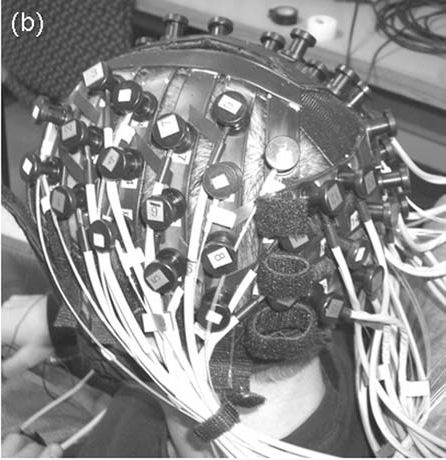
\includegraphics[width=4in]{laser.png}
\caption[Laser NIRS System]{Picture of a probe used in a Laser NIRS system. Note that this is not the system described above. \cite{fran06}}
\end{figure}

\section{The MCP II}

The MCP II is a versatile, multi-channel NIRS instrument. It was designed in order to map neuronal activation in neonatal and adult brains in response to motor, tactile, and visual stimulation. It aimed to have high SNR, good spatial sampling, and good clinical useability and ease of transportation \cite{wolf05}.

The MCP II used three LEDs to calculate the change in concentration of oxyhaemoglobin and deoxyhaemoglobin, opposed to the more common dual wavelength approach. They also used PIN photodiode's with a very large activation area, with 7.5mm$^2$, as their detectors. This is a very good idea. PIN photodiodes are especially sensitive, but with the addition of the large activation area it allows for a higher SNR \cite{wolf05}. 

The sensor designed in this system is fairly interesting. A flexible sensor that was molded with a curvature was used to fit neonatal heads as well as adults. Silicon and SMD devices were used to prevent light leakage. Transparent silicon was also placed around the photodiodes to provide two optical windows \cite{wolf05}.

The system is such designed that it is able to use 8 sensors at one time, with the ability to simultaneously measure the light intensity at two detectors. The system uses time multiplexed data acquisition with an oversampling ADC of 12-bits, to achieve a 100Hz sampling rate. Interestingly, the system is coupled to a stimulation unit that provides tactile, acoustic, and visual stimuli to the patient to accurately measure brain activity \cite{wolf05}.

The MCP II achieved very good results, obtaining a high SNR, high sensitivity, good resolution, and a good clean signal, as can be seen in Figure 2.2. Additionally, it is very convenient to have a multi-channel system that can simultaneously capture two channels \cite{wolf05}.

\begin{figure}[htp]
\centering
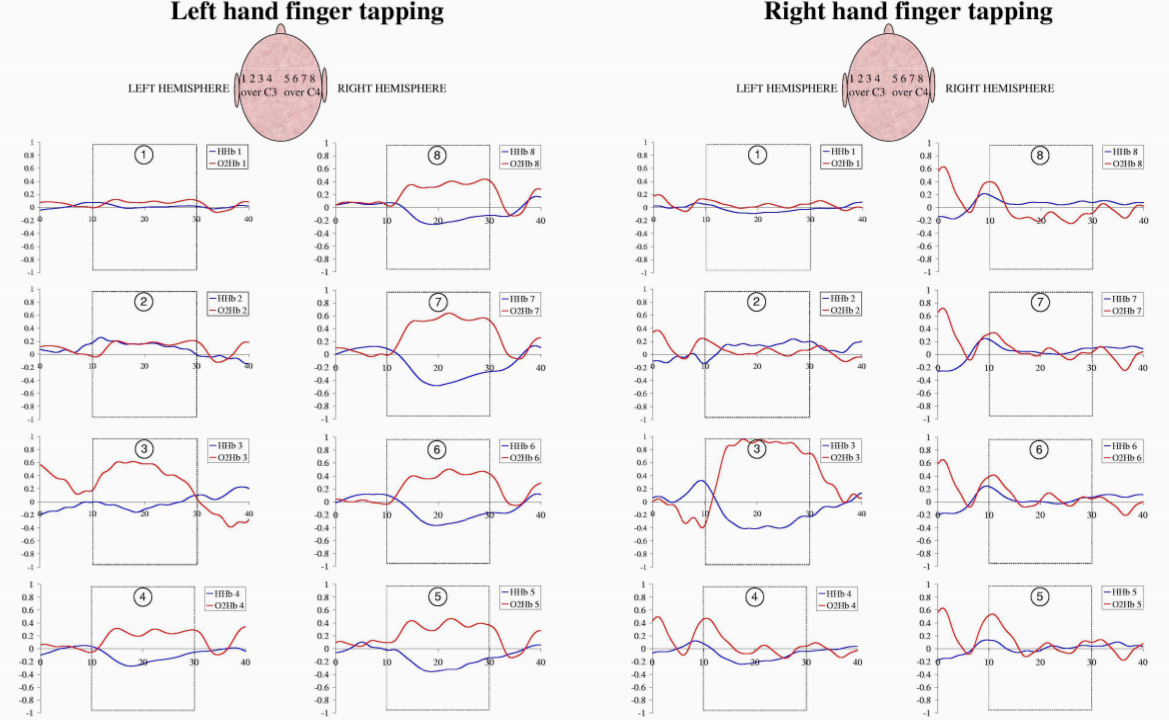
\includegraphics[width=6in]{mcp_t.png}
\caption[MCP II Measuring Motor Movement]{The MCP II measuring brain activity in the motor cortex in relation to finger tapping. "Finger tapping exercises were performed from second 10 to 30 (dotted box). The first (sensors 1-4) and the second column (sensor 5-8) measured over left and right hemisphere respectively before, during, and after left hand finger tapping. The third (sensors 1-4) and fourth column (sensor 5-8) show the left and right hemisphere during right hand finger tapping. An activation typically consists of an increase in oxyhemoglobin (O2Hb) concentration and of a decrease in deoxyhemoglobin (HHb) concentration. The higher O2 consumption in the activated area is immediately overcompensated by an increase in blood flow, which leads to the observed pattern. Both hands showed a stronger contralateral activation on the motor cortex hemisphere. The ordinates are scaled to μ mol/l." \cite{wolf05}}
\end{figure}

While, the MCP II is this projects main influence, it does have some downfalls. The system is using an unnecessarily powerful processor, running Linux, just to provide wired network communication. A simple pic18 can be used to provide network communication and be much cheaper. Additionally, the system is wired, making the system not very portable. Additionally, while the system is 'portable', it is more less transportable, rather than portable. Due to the number of channels used and the complexity of the system, it is fairly large, though comparatively small compared to Laser NIRS systems. The ideas used in the system are not original, but they successfully chose a myriad of good ideas to implement an excellent working system.

\section{Wireless Miniaturized NIRS System}

There have been similar LED based system designed that are wireless, smaller, and lighter. These designs are basically simplified designs of the MCP II,  while producing comparable results to other NIRS systems. One such design is \cite{mini08}. The main aspect of this design was to produce an lightweight, small, wireless NIRS system to minimize distress when imaging neonatal infants.

The design is simple and efficient using a dual wavelength LED design. It uses a an Silicon Labs 8051 type microcontroller connected to a Bluetooth module for communication. It is also multi-channel based system the ability to connect up to 12 channels, though only four are connected in the literature \cite{mini08}.

The sensor design, though not ideal, is unique. They grouped together multiple LEDs of the same wavelength to obtain a high integration density. Additionally, black epoxy was placed around each photodiode and LED group to prevent light contamination and leakage. The sensor placement is odd however, having two channels facing opposing directions as the other two. This is perhaps the drawback of their design \cite{mini08}.

They are able to obtain decent performance however, obtaining comparable results to that of MCP II, as can be seen in Figure 2.3.

\begin{figure}[htp]
\centering
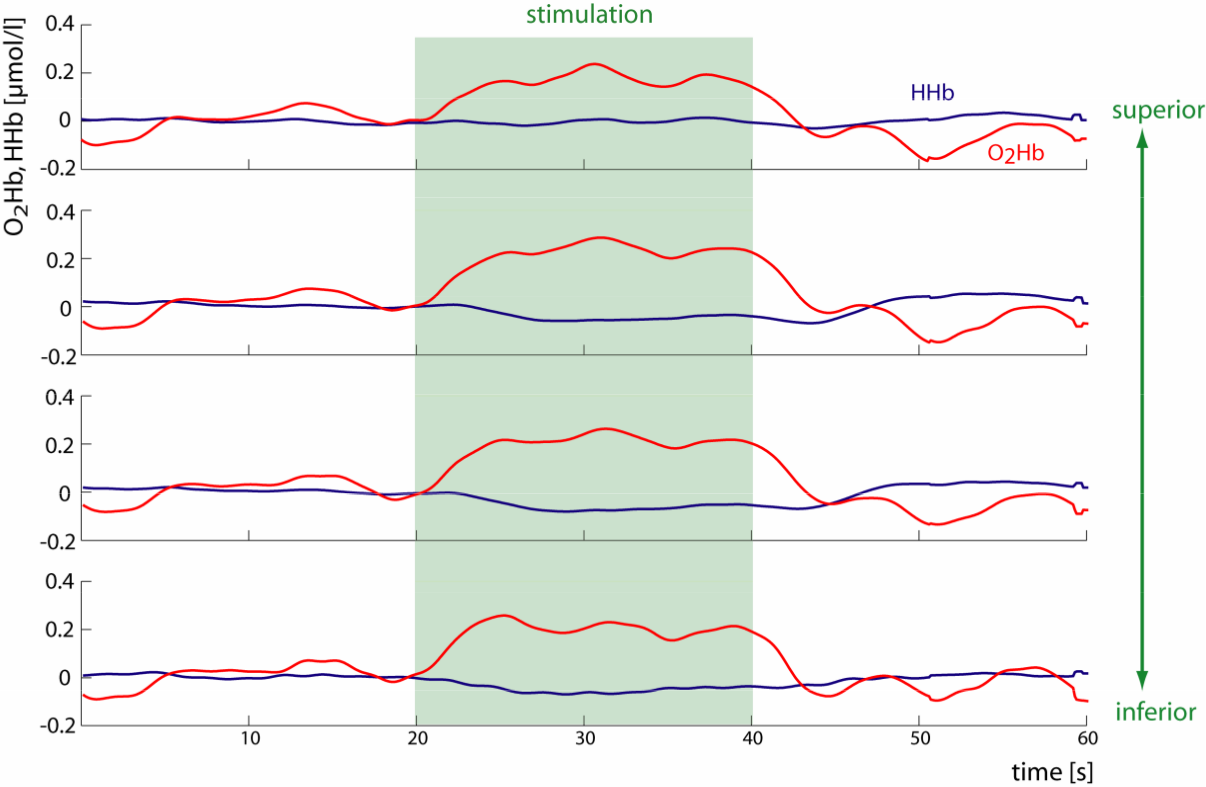
\includegraphics[width=6in]{mini.png}
\caption[Wireless Miniaturized NIRS System Measuring Motor Movement]{TheWireless Miniaturized NIRS System measuring brain activity in the motor cortex in relation to finger tapping. "Averaged hemodynamic response of the cortex to finger tapping for four source-
detector positions." \cite{mini08}}
\end{figure}                  % the first chapter
        \setcounter{figure}{0}
        \setcounter{equation}{0}
        \setcounter{table}{0}

  \chapter{Theory}

Clearly the main problem in this project is obtaining the haemodynamic signal from the signal light intensity measured by the photodiodes. Or, rather, turning near infrared light into the measurement of brain activity.

\section{The Basics}

Analyzing the absorption spectra of light shows that the main absorbers in the near infrared light range (700nm - 900nm) are blood chromophores of oxyhaemoglobin (oxygenated haemoglobin, O$_{2}$Hb) and deoxyhaemoglobin (deoxygenated haemoglobin, HHb). Water and lipids absorb very little light, they are negligible and are basically transparent to near infrared light as depicted in Figure 3.1. Additionally it can be seen that in this spectral range, light is weakly absorbed by the tissue, making this spectral range ideal for NIRS imaging, which relies on reflected (backscattered) light. Thus, any changes in light intensity shone into the body can be interpreted as varying concentration levels of O$_{2}$Hb and HHb. These varying levels of oxygenation are used to estimate blood volume and tissue oxygenation, which indicate haemodynamic activity \cite{rosen05}.

\begin{figure}[htp]
\centering
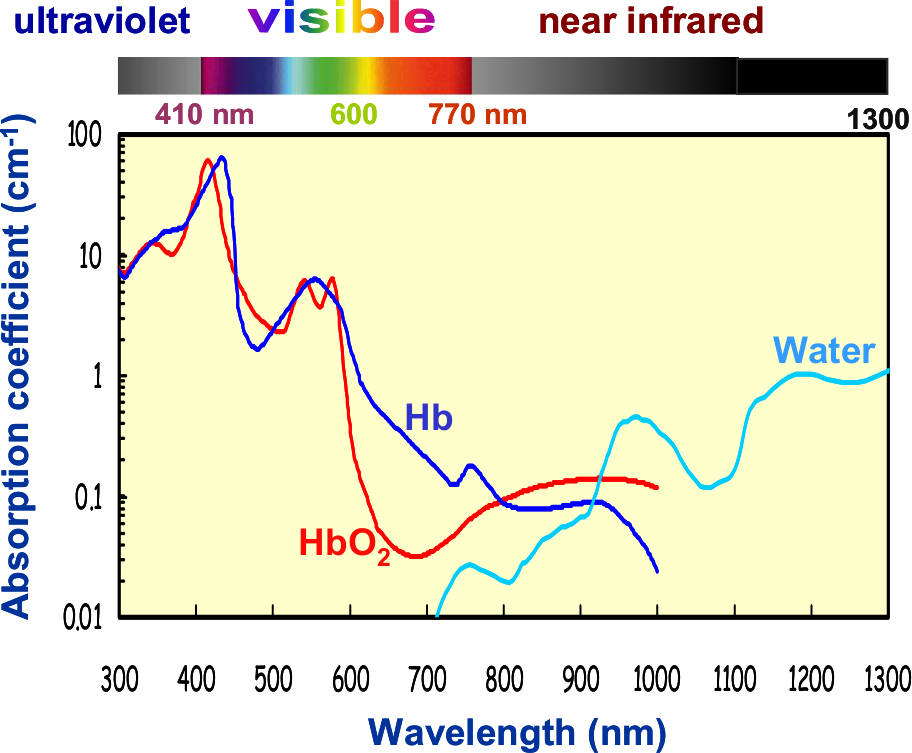
\includegraphics[width=4in]{spectra.png}
\caption[Propagation of photons]{Absorption spectra of deoxyhemoglobin (Hb), oxyhemoglobin (HbO$_2$), and water. The concentrations of Hb and HbO$_2$ are set to 50 μM$^1$.}
\end{figure}

\footnotetext[1]{Sergio Fantini’s Group, "Near-infrared spectroscopy for the study of biological tissue," Department of Biomedical Engineering, Tufts University, retrieved from http://ase.tufts.edu/biomedical/research/Fantini/researchAreas/NearInfraredSpectroscopy.pdf}

Near Infrared Light photons that are shone into the scalp are either absorbed by varying layers of tissue, such as the skin or the skull, scatter due to interactions with the tissue, or pass right through. Some of these scattered photons follow a kind of banana pattern through the head and back out due to the scattering effect of tissue (refer to figure 3.2). These backscattered photons can be picked up by a photodiode or a similar component \cite{rosen05}. However, now arises the problem of turning the measured light intensity into varying concentration levels of O$_{2}$Hb and HHb.

\begin{figure}[htp]
\centering
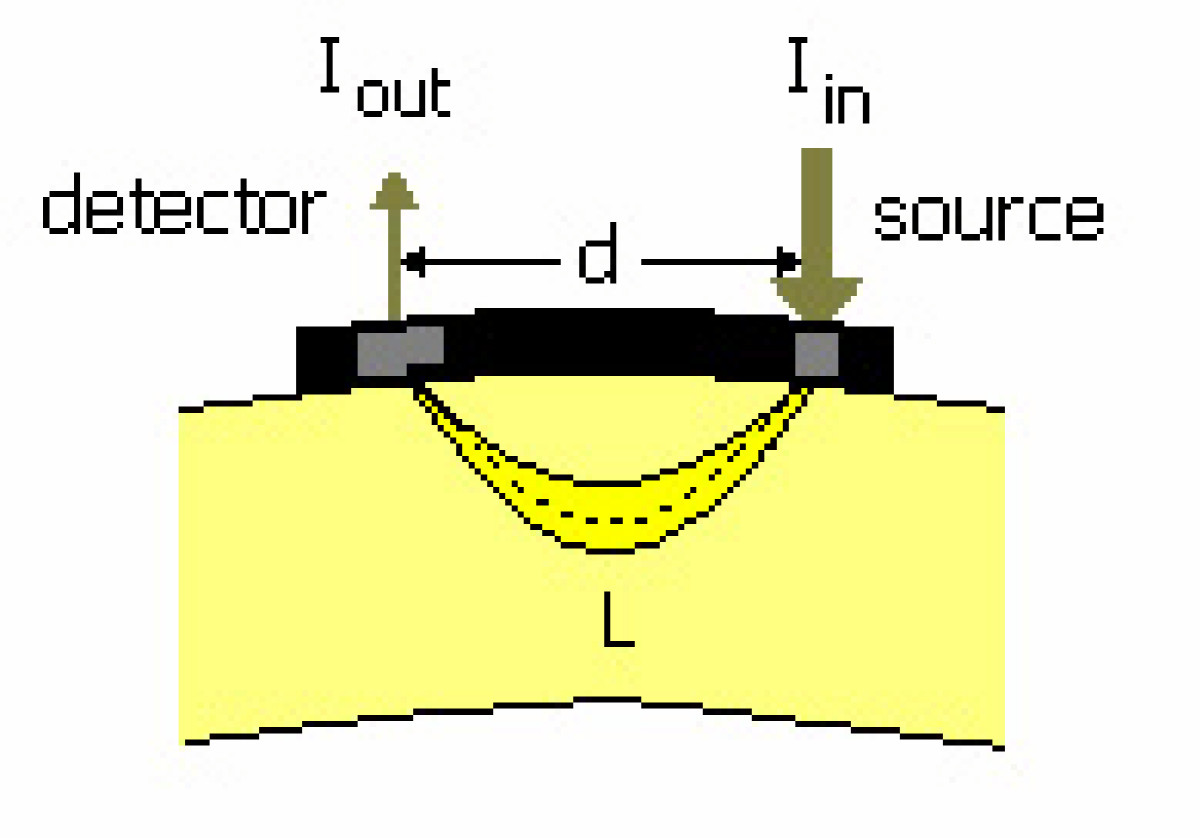
\includegraphics[width=4in]{banana.jpg}
\caption[Propagation of photons]{Propagation of photons from source to detector. The banana scattering pattern can clearly be seen here. \cite{rosen05}}
\end{figure}

\section {Modified Beer-Lambert Law}

This banana scattering effect is best described by the modified Beer-Lambert Law. The original Beer-Lambert law, A$^\lambda$ = $\epsilon^\lambda$cL, states the absorption of light (A) is proportional to the concentration of the absorber (c) multiplied by the specific wavelength extinction coefficient of the absorber ($\epsilon^\lambda$) and the path length the light has to travel (L, can be seen in Figure 3.2). However, this law only holds if the photons are absorbed or pass through the tissue in a straight line directly to the detector. Due to higher substance concentrations and substantial light scattering, the law does not hold in NIRS brain imaging \cite{chance97}. 

The modified law has to take into account the longer distance of light travel and loss of light intensity due to scattering. However, taking these into account would no longer purely calculate the amount of light absorbed. Rather it would find the amount of light absorbed and scattered or the total attenuation of the light, more accurately called optical density which varies for a different wavelength (OD$^\lambda$) \cite{rosen05}. Thus, introducing signal loss due to light scattering (G), the modified Beer-Lambert law becomes OD$^\lambda$ = $\epsilon^\lambda$cL + G. However, accurately measuring the path length of the light requires expensive highly specialized instruments. Thus, the pathlength the light has to travel can be estimated rather well by the distance between the light source and photodetector and the wavelength dependent differential pathlength factor (DPF$^\lambda$). That is,

\begin{equation}
L = d DPF^\lambda
\end{equation}
 
where d is the distance from the light source to the photodetector (refer to Figure 3.2) \cite{rosen05}. Assuming there is a constant light scattering loss, taking the average of two subsequent measurements the signal loss due to scattering (G) averages out. Producing the modified Beer-Lambert law this project is based on \cite{chance97}.

\begin{equation}
\Delta OD = \epsilon^\lambda c d\ DPF^\lambda
\end{equation}

Given the modified Beer-Lambert law, the light intensity measured by the photodiode in NIRS can accurately be described by 

\begin{equation}
I = I_{emitted} e^{-OD^\lambda}
\end{equation}

where I$_{emitted}$ is the light emitted by the light source into the head \cite{wolf05,rosen05}. Rearranging this equation gives

\begin{equation}
OD^\lambda = \ln \frac{I_{emitted}}{I}
\end{equation}

Taking the average of the optical density (or attenuation) between two subsequent measurements gives the equation

\begin{equation}
\Delta OD =  \ln \frac{I_{emitted}}{I_2} -  \ln \frac{I_{emitted}}{I_1} = \ln \frac{I_1}{I_2} = \epsilon^\lambda c d\ DPF^\lambda
\end{equation}

where I$_1$ is the first measurement and I$_2$ is the subsequent measurement \cite{yam02}. Since it is well documented that the main chromophores in blood that react to the near infrared light spectra are oxyhaemoglobin and deoxyhaemoglobin, finding the optical density in these cases is described by

\begin{equation}
\Delta OD = \ln \frac{I_1}{I_2} = (\epsilon^\lambda_{O_{2}Hb}\Delta c^\lambda_{O_{2}Hb} + \epsilon^\lambda_{HHb}\Delta c^\lambda_{HHb})  d\ DPF_\lambda
\end{equation}

where $\Delta$ c is the change in concentration of the specific chromosphore \cite{eke06}. Now if the attenuation of light (Optical Density) is measured at two different wavelengths $\lambda$1 and $\lambda$2, the above equation can be rearranged to yield

\begin{equation}
\Delta c_{O_{2}Hb}  =  \frac{\epsilon^{\lambda 1}_{HHb} \ \left (\frac{\displaystyle \Delta OD^{\lambda 2}}{\displaystyle d DPF^{\lambda 2}} \right) - \epsilon^{\lambda 2}_{HHb} \ \left (\displaystyle \frac{\Delta OD^{\lambda 1}}{\displaystyle d DPF^{\lambda 1}}\right)}{ \epsilon^{\lambda 1}_{HHb}\epsilon^{\lambda 2}_{O_{2}Hb} - \epsilon^{\lambda 2}_{HHb}\epsilon^{\lambda 1}_{O_{2}Hb}}
\end{equation}

\begin{equation}
\Delta c_{HHb}  =  \frac{\epsilon^{\lambda 1}_{O_{2}Hb} \ \left (\frac{\displaystyle \Delta OD^{\lambda 2}}{\displaystyle d DPF^{\lambda 2}}\right) - \epsilon^{\lambda 2}_{O_{2}Hb} 
\left (\frac{\displaystyle \Delta OD^{\lambda 1}}{\displaystyle d DPF^{\lambda 1}}\right)}{\epsilon^{\lambda 1}_{O_{2}Hb}\epsilon^{\lambda 2}_{HHb} - \epsilon^{\lambda 2}_{O_{2}Hb}\epsilon^{\lambda 1}_{HHb}}
\end{equation}

giving us the change in concentration between two measurements for oxyhaemoglobin and deoxyhaemoglobin \cite{eke06,yam02}. This can further be extended to find oxygenation of the blood and blood volume \cite{rosen05};

\begin{equation}
OXY = \Delta c_{O_{2}Hb} - \Delta c_{HHb}
\end{equation}

\begin{equation}
BV = \Delta c_{O_{2}Hb} + \Delta c_{HHb}
\end{equation}

It is important to note however the modified Beer-Lambert law used to derive the above equations is based on two assumptions: the absorption of the tissue changes homogeneously, and the light intensity lost due to scattering is constant. These assumptions are not true in practice. However, with appropriate wavelength selections for the light sources, these errors are minimal and negligible \cite{eke06}s.

It has been shown in past studies that brain activity as a result of a specific stimulation produces a highly localized increase in local oxygen consumption directly followed by an increase in blood flow within a few seconds, changing the O$_{2}$Hb and HHb concentrations \cite{freeman03}. Thus, we can conclude that changes in O$_{2}$Hb and HHb relate to brain activity.                  % the first chapter
        \setcounter{figure}{0}
        \setcounter{equation}{0}
        \setcounter{table}{0}

  \chapter{Design Procedures}

To create the NIRS system, a sensor consisting of LEDs, to emit light through the area of interest, and photodiodes, to convert the transmitted incident light into an electrical signal, must be made. The signal from the photodiodes must then be connected to an ADC in order to convert the analog signal to a digital signal that is readable by the computer doing the calculations. The digital signal must then be transmitted to the computer where calculations would be done.

To control the LEDs and convert the analog signal to a digital one, a microcontroller will be used. The microcontroller will then be interfaced to a computer through UART, initially through USB, then finally wirelessly through Bluetooth. The overall system can be seen in Figure 4.1.

\begin{figure}[htp]
\centering
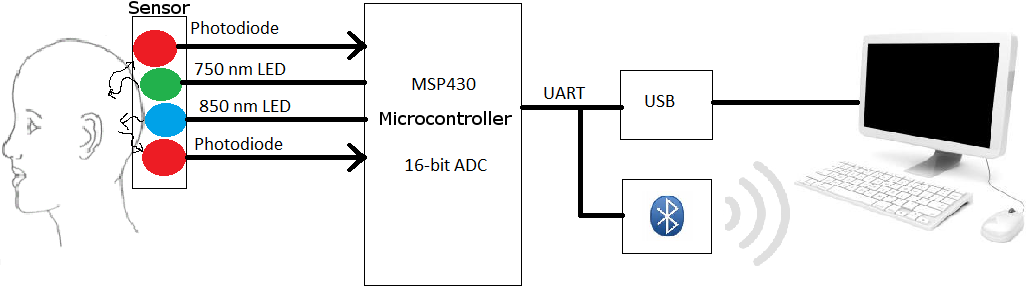
\includegraphics[width=6in]{design.png}
\caption[A very basic overview of the system.]{A very basic overview of the system. For the testing phase, USB will be used to communicate with the computer. Eventually, Bluetooth will be used as the primary means of communication.}
\end{figure}

Bluetooth was selected over a low power wireless interface, such as ZigBee, due to Bluetooth being widely available on all modern phones. It was the intention to interface the device with a mobile phone, time permitting. However, this was never done. Bluetooth consumes much more power than other competing wireless communication systems, so to obtain optimum battery life it is not ideal. Had the author realized that there would be no time to interface the device with a mobile phone, a lower power wireless communication system would have been selected, most probably ZigBee.

To design the NIRS system, it was decided to design everything from scratch. The microcontroller circuit, the sensor, as well as the software was designed and built/written. This was done to truly test the author's knowledge obtained from his years at McMaster University. Additionally, this project provided an excellent chance to be introduced to microcontroller circuit design.

Development of this system began with the microcontroller, since nothing would work without it, followed by the sensor, then finally the software.

\section{The Microcontroller}

The microcontroller selected for use in this project is the Texas Instruments MSP430, specifically the MSP430f4250. The MSP430 was chosen due to its low power requirements and 16-bit sigma-delta ADC. In most cases, a 12-bit ADC would be sufficient, but a higher resolution will allow for the weak temporal signals to be detected easier. The MSP430 is also fairly cheap. These characteristics make it ideal for this project and made it standout from other competitors. 

While the MSP430f4250 is slightly excessive for this project, due to its built in LCD controller and array of I/O ports, it was the cheapest MSP430 model that the minimum required I/O ports and a 16-bit ADC.

While the MSP430f4250 does not have any dedicated UART hardware on-board, a software timer UART is sufficient in this project. The project only requires samples to be transmitted from the microcontroller to a computer. It was decided that flow control was not necessary for this project. This decision, however, led to many problems during testing, which will be discussed later. 

To design the microcontroller circuit, datasheets, user guides, application notes, and reference designs were read and used as a basis. Thankfully, the MSP430 has many built in capacitors and resistors (for example, adjustable oscillator capacitors) that help to reduce the overall components of the  build. The schematic of the device can be seen in Figure 4.2

\begin{figure}[htp]
\centering
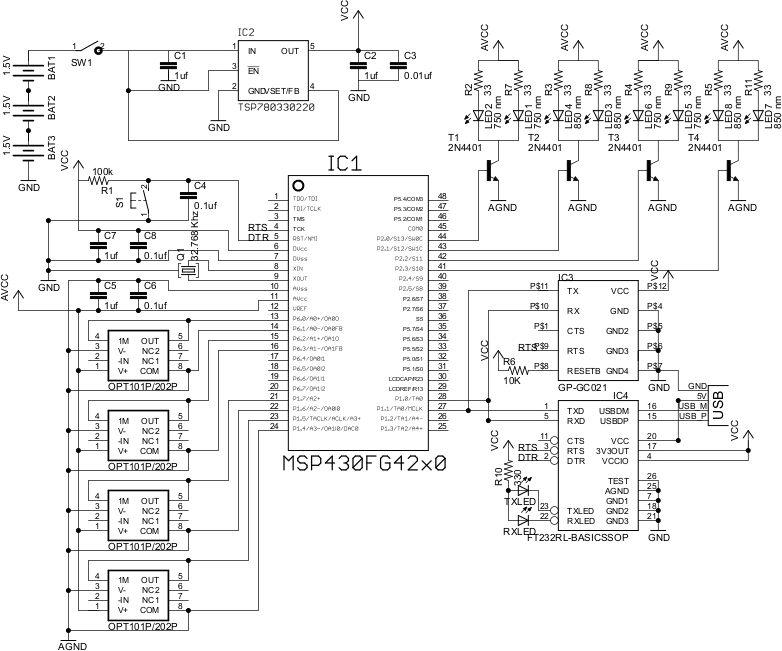
\includegraphics[width=6in]{mcu.png}
\caption[Schematic of the system]{The schematic of the overall system. Note that two sensors are included in the diagram. The TPS79433 LDO regulator was used instead of the TPS780330220 in the diagram}
\end{figure}

A 32.768 Khz crystal is used because that is the only crystal the MSP430f4250 is designed to use. It is used as somewhat as a watchdog timer, waking the MSP430 up at select intervals to see if there is work to be done, unless it is told otherwise. Capacitors between VCC and GND were placed as close the the microcontroller as possible, as per Dr. Doyle's suggestion. This helps to reduce any noise that may have been picked up between the power supply and the microcontroller. This is especially a problem with the MSP430, any fluctuations/noise in the power supplied to it will cause the ADC to be very noisy. This is perhaps the main reason why the MSP430 is not very popular in projects that require signal acquisition. However, with proper consideration, this should not be much of an issue. To further reduce the noise in the ADC, separate power and ground are used for digital signals and analog signals, VCC \& GND and AVCC \& AGND respectively. 

The frequency the microcontroller operates at is governed by the voltage supplied by its power supply. Since the Bluetooth module operates at 3.3V and the USB UART device outputs power at 3.3V when powered by USB, a 3.3V power supply was selected. This sets the frequency of the microcontroller to ~7 Mhz, which is set by a FLL (frequency-locked loop). The speed the microcontroller operates at is of no big importance in this project. The sampling rate for data acquisition is slow enough, at 100Hz, that the 32Khz crystal is fast enough to supply the clock at which to sample the data. The speed of the UART is what is affected by the microcontroller speed. It was determined that the speed of the UART must be at least 76 800 bit/s or 76.8k baud (see Appendix A), which is easily exceed with a clock ~7Mhz.

To supply this voltage, 3 AA batteries connected to a regulator were chosen for long battery life. An LDO (low-dropout) regulator was selected over a more traditional regulator, such as an LM317. An LDO regulator was chosen because LDO regulators are highly efficient, consume very little power, and have low quiescent current, increasing battery life. Due to the the low power-requirements of every component, not much current is required by the system, making an LDO regulator ideal for use. LDO regulators are limited to the amount of current they can output due to consuming very little power.

The LDO regulator selected to do the job is the Texas Instruments TPS79433. It outputs voltages at 3.3V at a maximum current of 250mA. Additionally, it can be supplied power at less than 3.3V and will still output power at 3.3V. This is a nice feature because when the batteries drain to below 3.3V, the unit will still be operational. This regulator was selected because it meets all the requirements and free samples were obtainable from Texas Instruments. The circuit for the power supply was derived from the datasheet. 

To interface with the computer, the an USB to UART device was used. The FTDI FT232 was selected due to many good reviews on the device and good compatibility with Linux and Windows. The circuit design is based on the reference design given in the datasheet. One thing to note is that, while the built-in bootloader implemented flow control, which was necessary to invoke the bootloader, the software UART used in this project did not. As such, the DTR wire had to be disconnected from the microcontroller when not programming the device. Otherwise, the DTR wire would reset the device when communicating with the computer. The USB UART interface was used to program the device and initially communicate to the device during testing.

Once everything was deemed working, the Bluetooth module was added to interface with the computer. The Bluetooth module selected was RF-BTMX417 by MDFLY. This was selected due to its cheap price, Bluetooth 2.0 specifications, and low power requirements. The design for the Bluetooth module was based on the reference design in the datasheet.

Once all the parts were selected, the majority of the necessary parts were ordered from Digikey due to their cheap prices. Free samples were obtained of the microcontroller and LDO regulator from Texas Instruments. The Bluetooth module was ordered from ebay. The prototype was built on a breadboard using SMD to DIP adaptors for each component needing one. The prototype can be seen in figure 4.3

\begin{figure}[htp]
\centering
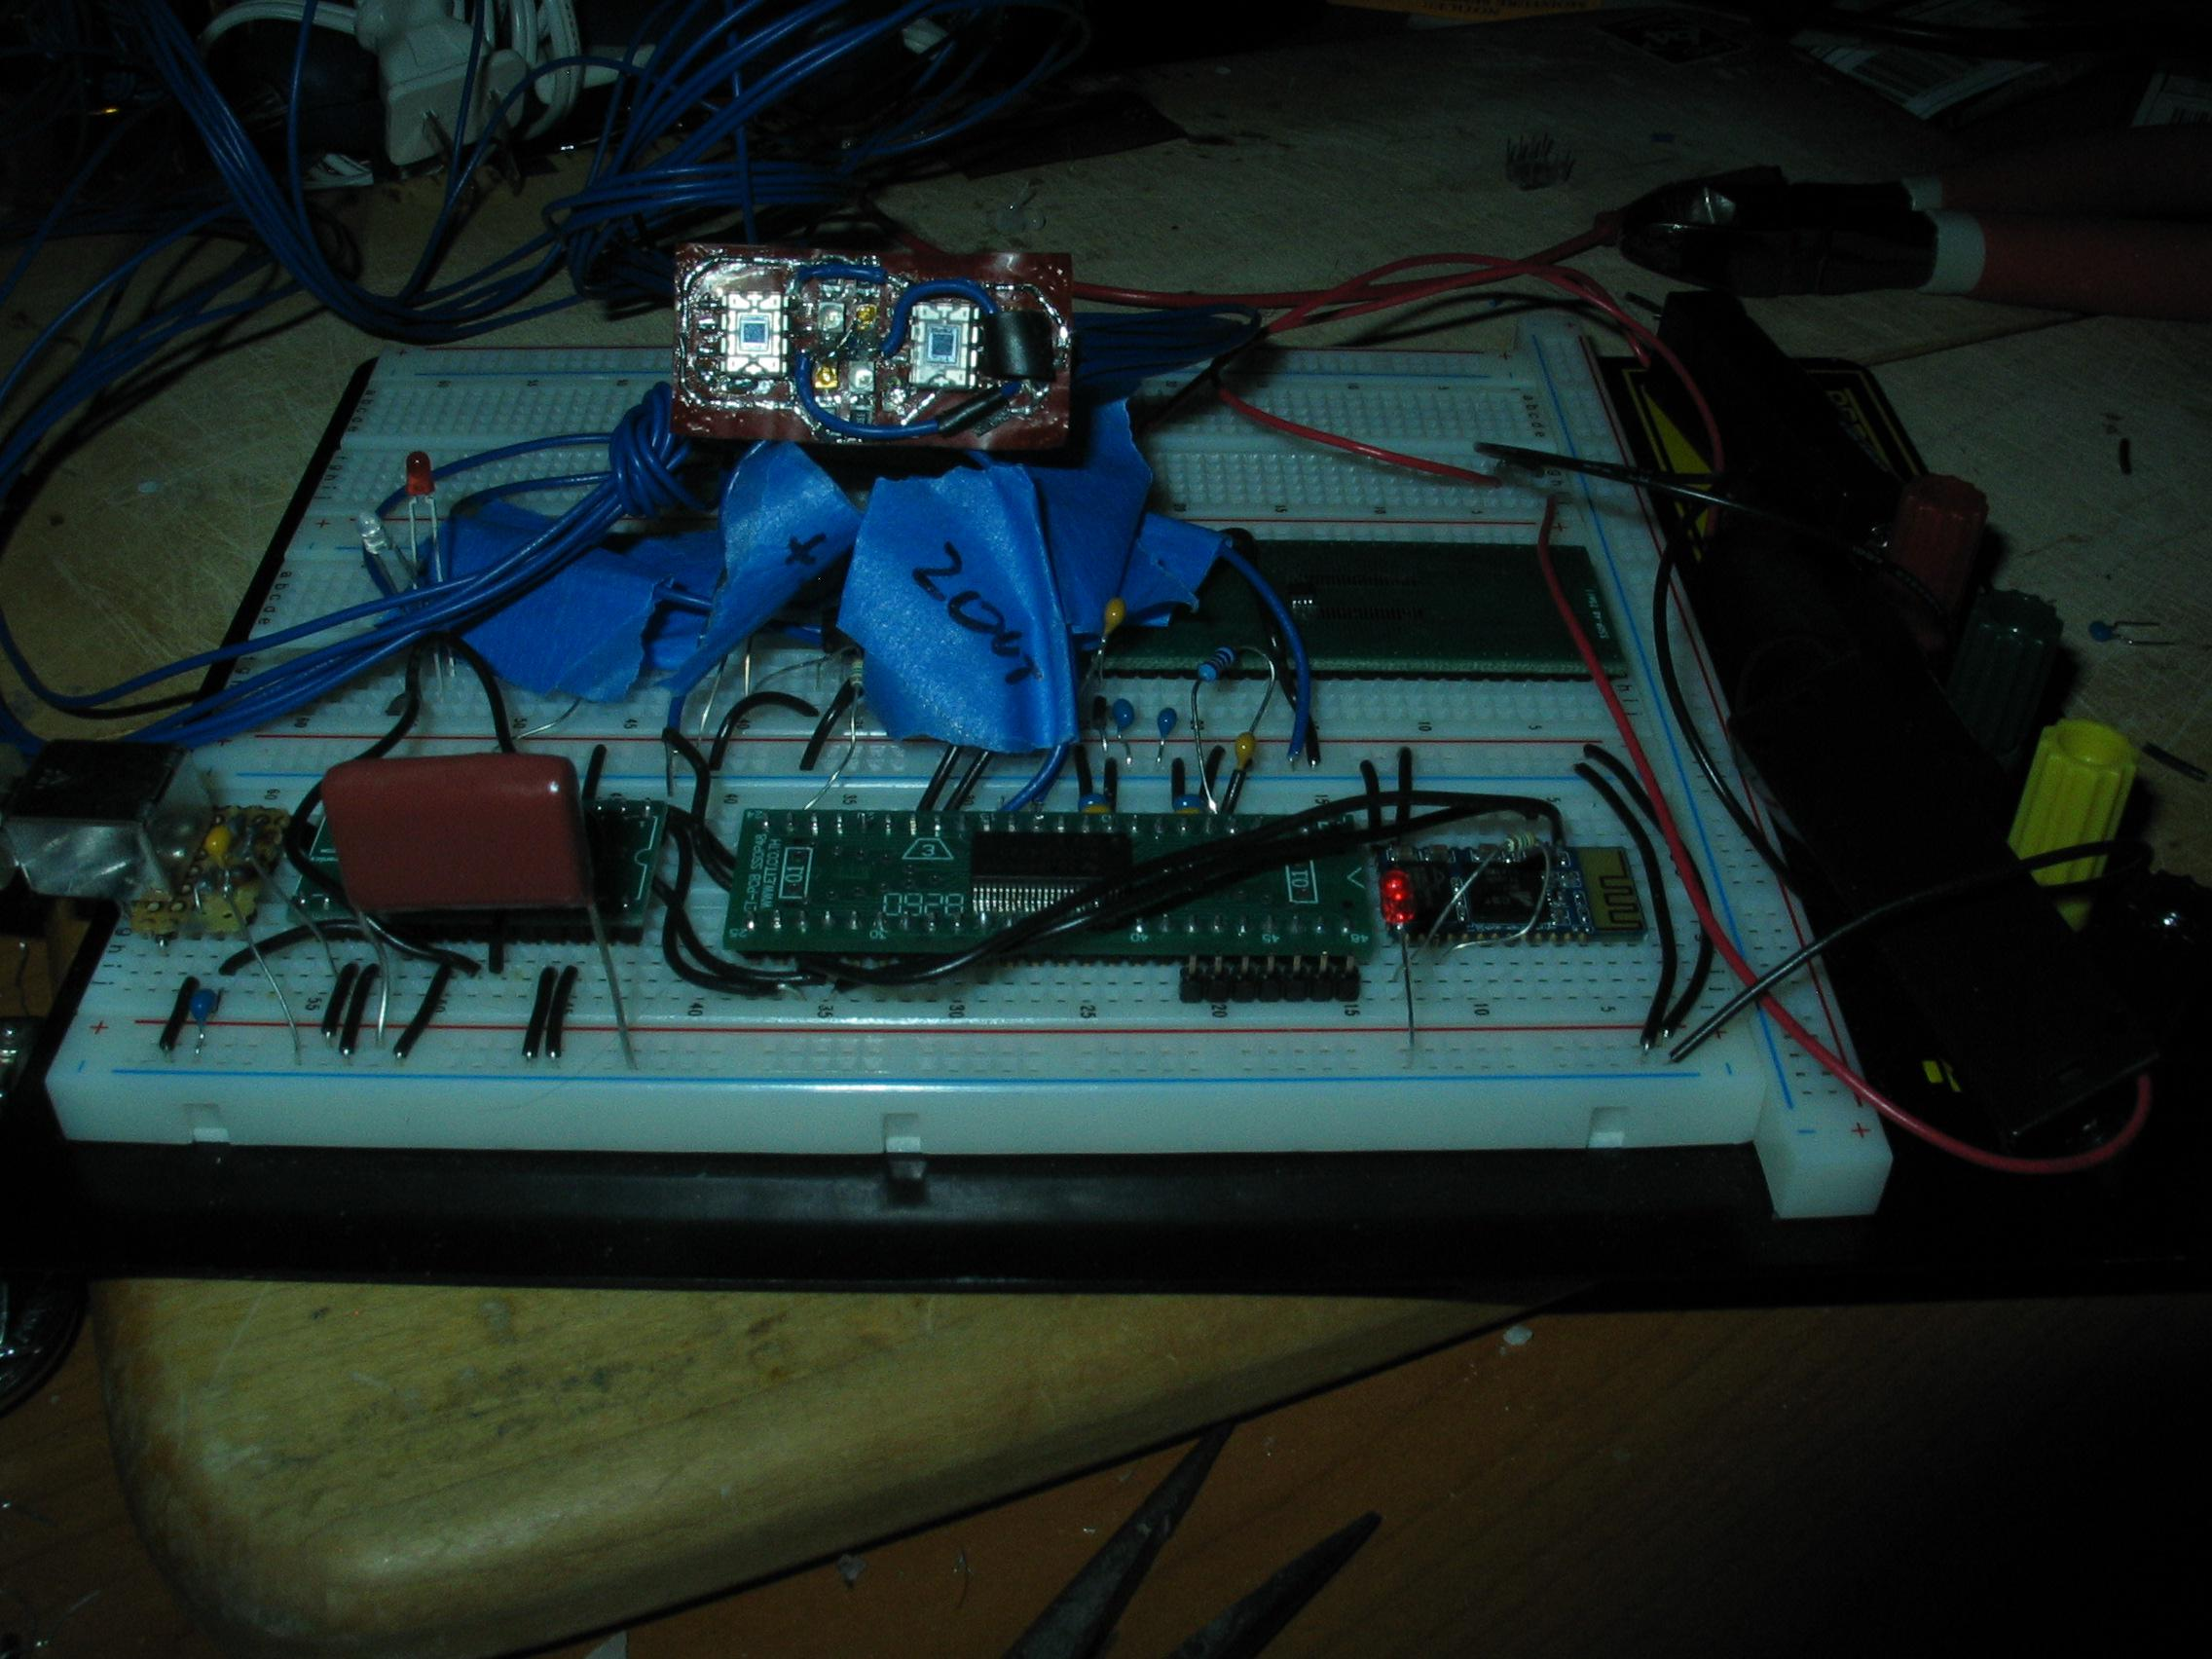
\includegraphics[width=6in]{prototype.jpg}
\caption[The Prototype]{Picture of the prototype}
\end{figure}


To program the device, the MSP430f4250 has a a built-in non-overwritable (without JTAG) bootloader that can be programming over UART. A JTAG programmer would have cost at least \$100, greatly increasing the cost of this project, though making debugging much easier. The mspgcc tools included software, written by developers at TinyOS, to write to the bootloader on the MSP430. The mspgcc toolchain was used to compile the software, specifically mspgcc-4.4.3, and then programed to the device using the TinyOS software.

\section{The Sensor}

The sensor was first designed by selecting the components. The main problem was sourcing the LEDs with the desired wavelengths. After many emails to various distributors and manufactures, it was discovered Marubeni Corporation sold 750nm SMD LEDs in low quantities. The epitex SMT750-25 to be exact. As such, 750 nm LEDs were selected as one light source.

The wavelength of the other LED light source, must be above 800nm and be such that it minimizes interference between the two LEDs. Based on the study done in [4], the LEDs with wavelengths of 750nm and 850nm were selected to minimize interference between each LED. The 750nm wavelength responds better to deoxygenation in the blood and the 850nm wavelength responds better to oxygenation in the blood. Luckily enough, the 850nm LEDs were easily sourceable from Digikey in SMD form. The OSRAM SFH4650 being the only 850nm LED easily obtainable, or rather only 800 - 870nm SMD LED easily obtainable. The OSRAM SFH4650 has very recently been replaced by the more efficient SFH4651, while still providing similar specifications.

Unfortunately, the spectral half width of the LEDs are broader than desired. The 750nm LEDs have a spectral half-width of $\pm$ 35nm. While the 850nm LEDs have a spectral half-width of $\pm$ 42nm. This means the effective wavelength may vary by the spectral half-width, causing cross-talk between the LEDs and possibly throwing off the calculations. They have narrow halfangles, however, $\pm$ 25$^\circ$ and $\pm$ 20$^\circ$, respectively, which is desired to limit light leakage and force the highest light intensity towards the area of interest. With a forward current of 100mA, it is assumed the approximate penetration depth of these LEDs is 1cm, based on past studies \cite{rosen05}.

The LEDs are the most power-hungry device in this system. They could not be directly driven by the microcontroller. NPN transistors were selected to do this task. Specifically, the 2N4401 600mA NPN general purpose transistor. The 2N4401 was selected as it was the cheapest transistor available at Digikey with greater than 200mA continuous collector current. Each led has a maximum forward current of 100mA, so to power the LEDs at their maximum intensity, a 200mA transistor would be needed. The microcontroller would turn the NPN transistor on when it was desired to turn its subsequent LED on. Setting the Base of the NPN transistor to high, would allow current to flow from the Collector to the Emitter. Setting the Base to low (GND), would stop the current from flowing from the collector to the emitter. For a high integration density, each sensor and each transistor would have 2 LEDs of the same wavelength. This can be seen in Figure 4.4.

\begin{figure}[htp]
\centering
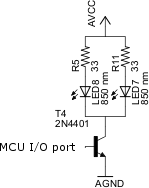
\includegraphics{led.png}
\caption[LED control diagram]{The schematic of controlling one wavelength of LED on the sensor}
\end{figure}

To detect the reflected light back, a photodiode must be used. However, the electrical signal measured by a photodiode varies in current, opposed to voltage as most ADCs work. As such, the current must be converted into corresponding voltage by a transimpedance amplifier. An interesting solution to this problem is the OPT101 by Burr-Brown. It is a monolithic photodiode with a built-in transimpedance amplifier, all in a small DIP-8 package. This makes it ideal for this project. Two photodiodes are placed on each sensor to pick up scattering and increase the overall surface area of the detectors.

The overall design of the sensor can be seen in Figure 4.5. It was decided that the transistors would be put on the PCB rather than on the sensor to reduce the size of the sensor.

\begin{figure}[htp]
\centering
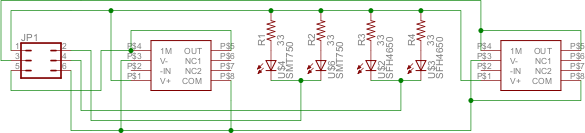
\includegraphics[width=6in]{sensor.png}
\caption[Sensor schematic]{The schematic of one sensor.}
\end{figure}

\subsection {Building the sensor}

Building the sensor was a daunting and hard task. The sensor had to be flexible to adhere to the head of the patient. As such, a flexible PCB is desired over a ridged one. 

To create the flexible PCB, the toner transfer method of homemade PCB creation was used. The PCB mill in the IEEE student Branch is not able to mill such a thin layer of copper on a flexible surface, and especially not with such thin tracings. 

The basic idea behind the toner transfer method is to print the design onto glossy paper using a laser printer. Melt the toner onto the copper board using an iron or something equally hot. Then etch the board using an enchant such as Ferric Chloride. Then to remove the toner from the PCB using a solvent such as acetone.

Dupont generously supplied a sample of dual sided Pyralux Copper PCB. However, making dual sided PCBs is no trivial task using the toner transfer method. My initial attempts to do so proved fatal. As such, one side was used a a ground plane, while the other side was etched. Since the LEDs were surface mount, all the devices had to be surface mount, unless they were to be mounted on the opposite side. 

To create the toner mask, Cadsoft EAGLE was used. The schematic was laid out in EAGLE, then the PCB designed. The idea was to minimize the size, keep the LEDs as close to the photodiodes as possible, and keep the parts somewhat symmetric to its double, while only making traces on one side. This layout sets the source-detector distance to be about 1cm (needed solve equations 3.7 and 3.8). The result can be seen in Figure 4.6.

\begin{figure}[htp]
\centering
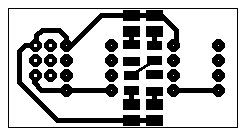
\includegraphics{sensorpcb.png}
\caption[Sensor pcb layout]{The pcb layout of the  sensor, not mirrored.}
\end{figure}

The layout was then mirrored and printed out onto thick glossy photo paper (Staples Photo Plus Gloss Paper to be exact) using a Brother laser printer with toner usage set to high. The Brother laser printer is all that I had on hand, an older model laser printer would have been ideal since the Brother laser printer toner have a high melting point, making it hard to melt the toner from the paper onto the copper. The glossy paper was then placed onto the copper board and ironed with a standard household clothes iron set to high. The iron was left on for about 15 minutes. After which, the iron was removed and the copper board placed into water to separate the paper from it. After about 10 minutes, the remaining paper was peeled off of the copper board by hand. 

The toner was now stuck to the copper board. Any broken traces were touched up with a Sharpie marker. The opposite side (the ground plane) was coloured black to prevent the enchant from eating away at it. The board was then submerged in the etching solution (Ferric Chloride) to remove the exposed copper. After about 20 minutes, the exposed copper was removed and the board fully etched. The board was then rinsed off in water and cleaned up with acetone to remove the toner and Sharpie marker from the board. Any extra copper traces were scraped off. Solder was placed onto the copper traces to prevent oxidation and make soldering the components easier. The PCB was then complete as can be seen in Figure 4.7.

\begin{figure}[htp]
\centering
\subfigure[Sensor after etching]{ 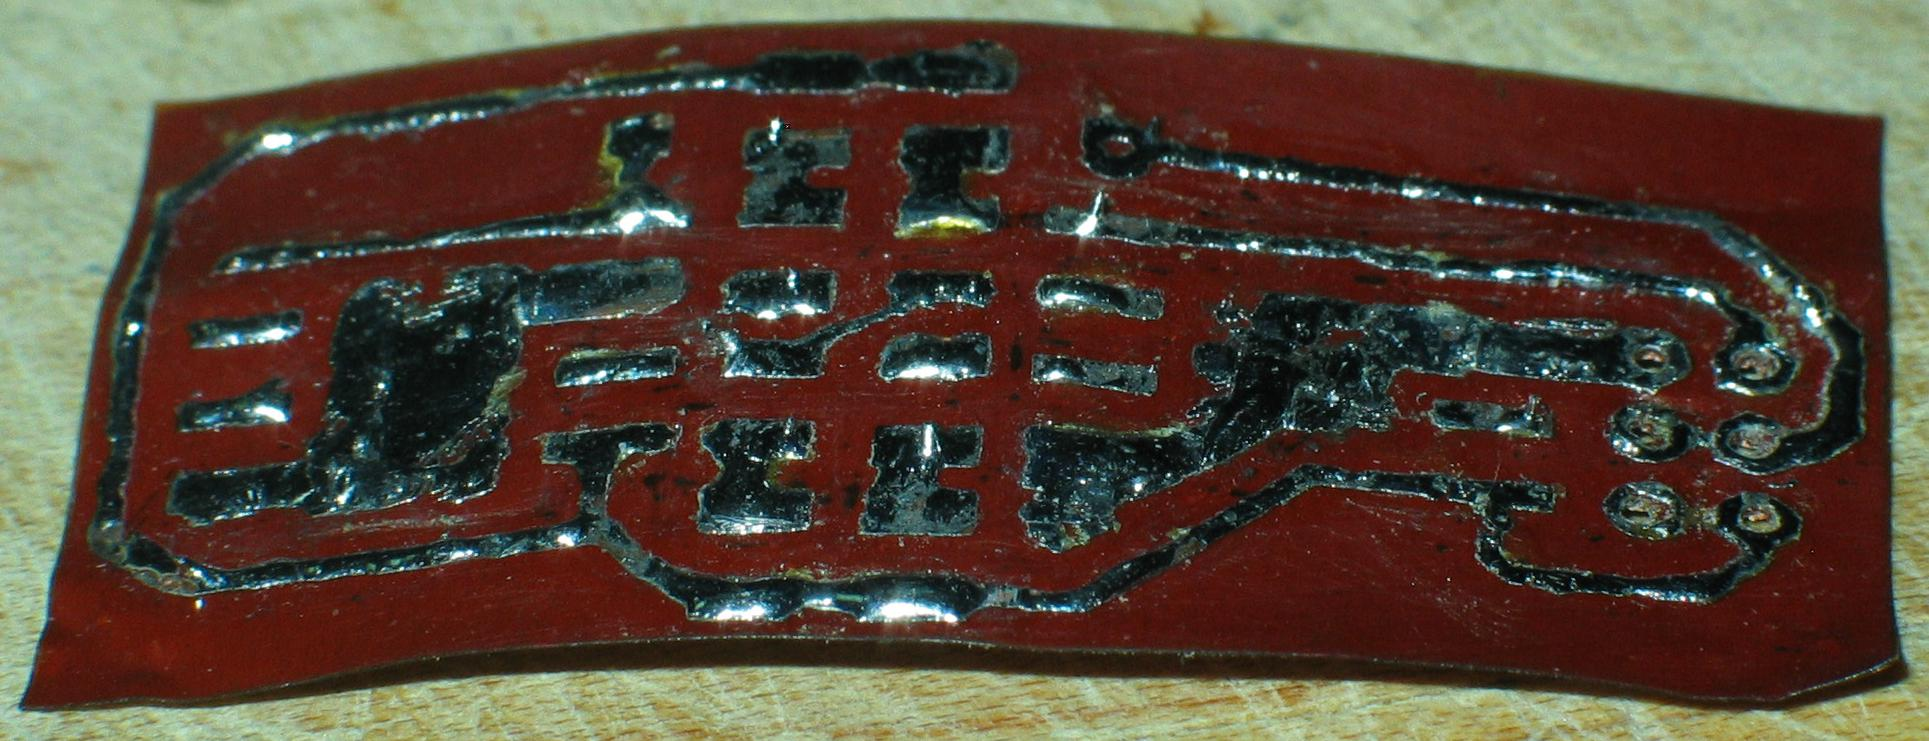
\includegraphics[width=6in]{sensorproto.jpg}}
\subfigure[Sensor showing flexibility]{ 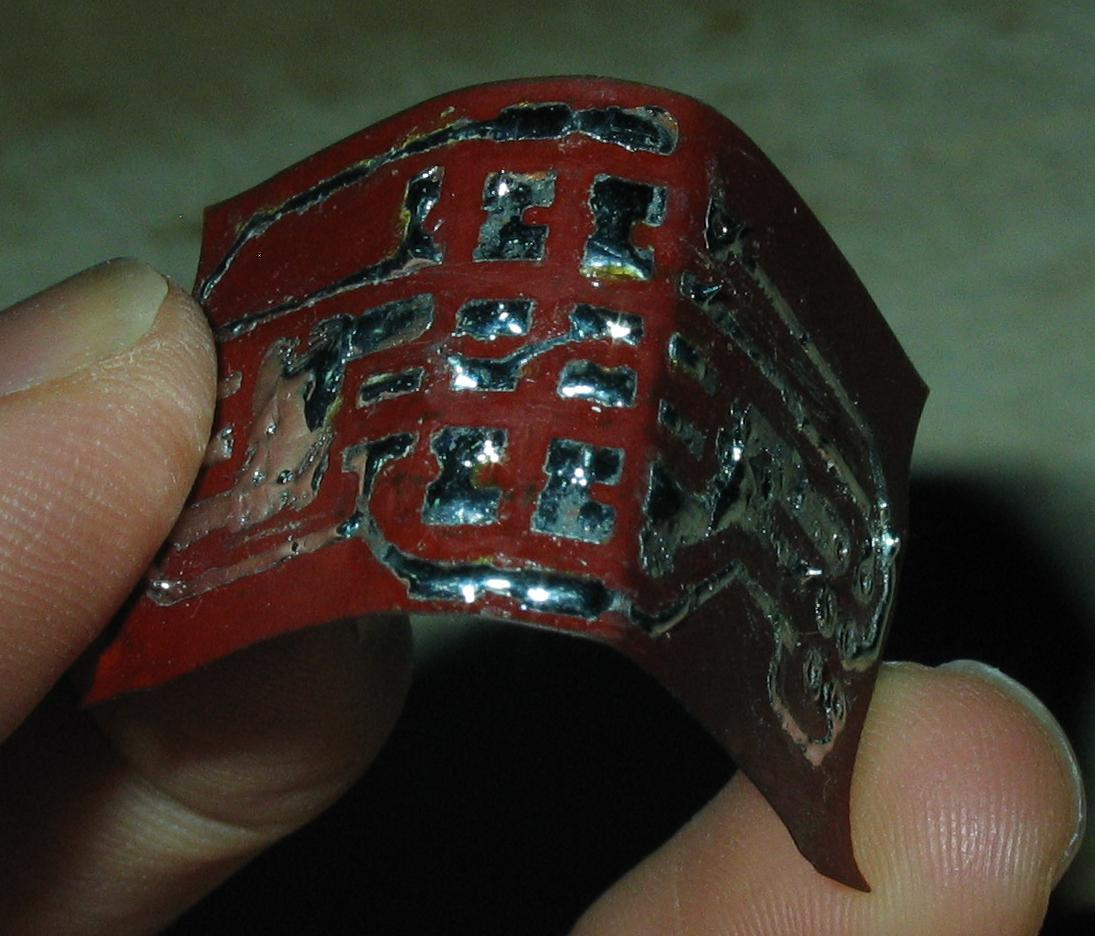
\includegraphics[width=6in]{sensorbend.jpg}}
\caption[Sensor prototype PCB]{The completed sensor PCB}
\end{figure}

Unfortunately, I made the traces to thin. While the came out okay out of the etchant, after many bends, some traces broke (even though they appeared fine). 

Again, the majority of the electrical components were obtained from Digikey. With the exception of the OPT101 monolithic photodiode, which was obtained from Texas Instruments as a free sample. After populating the sensor and difficult task of adding jumper wires, the finalized sensor prototype was complete. Correctly building the board took quite a few hours to complete. The complete sensor can be seen in Figure 4.8. Due to time constraints only 1 sensor was built. Though, the microcontroller was designed to handle 2.

\begin{figure}[htp]
\centering
\subfigure[Complete Sensor Prototype]{ 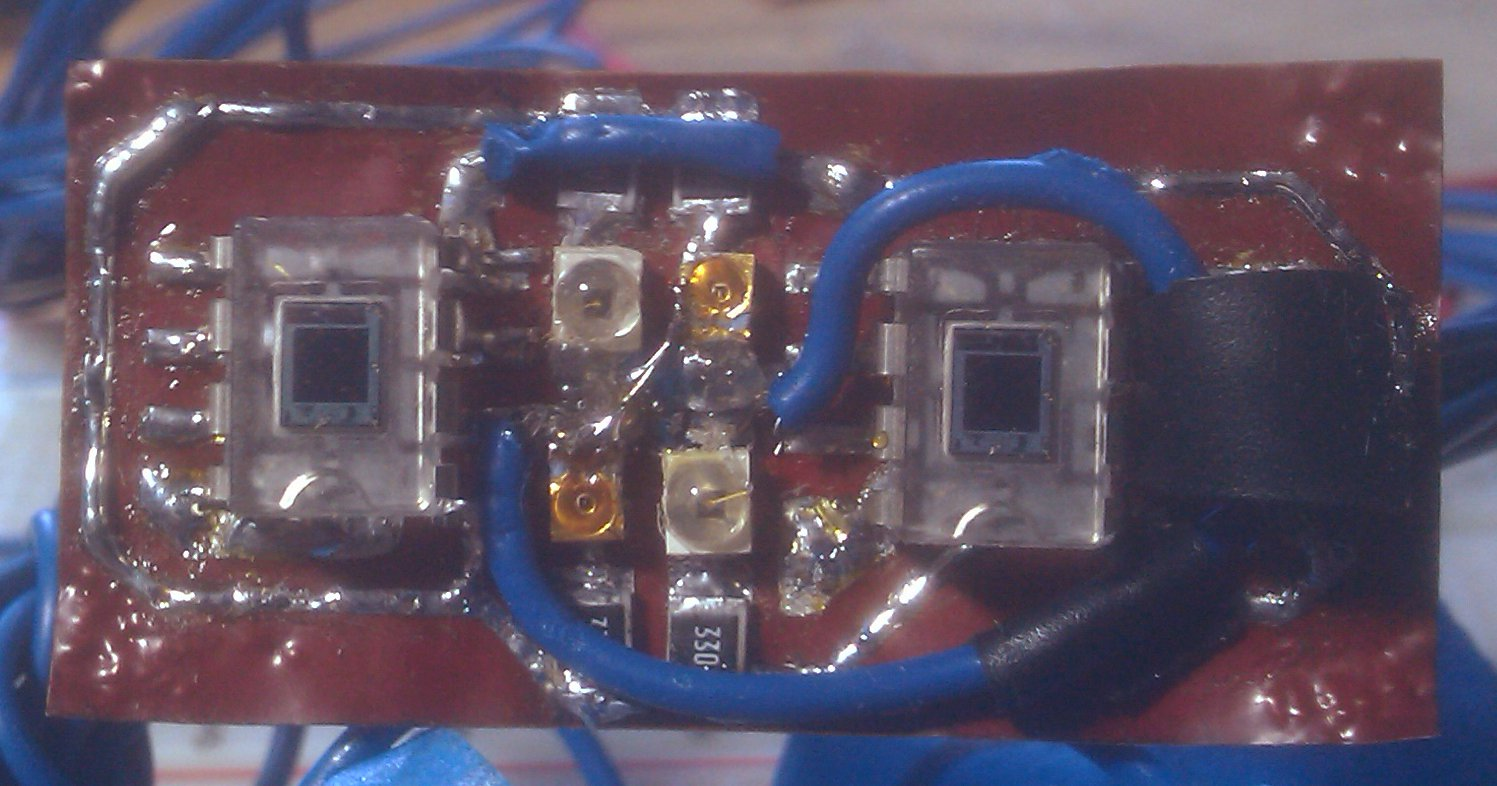
\includegraphics[width=6in]{csensorproto.jpg}}
\subfigure[Sensor Prototype showing flexibility]{ 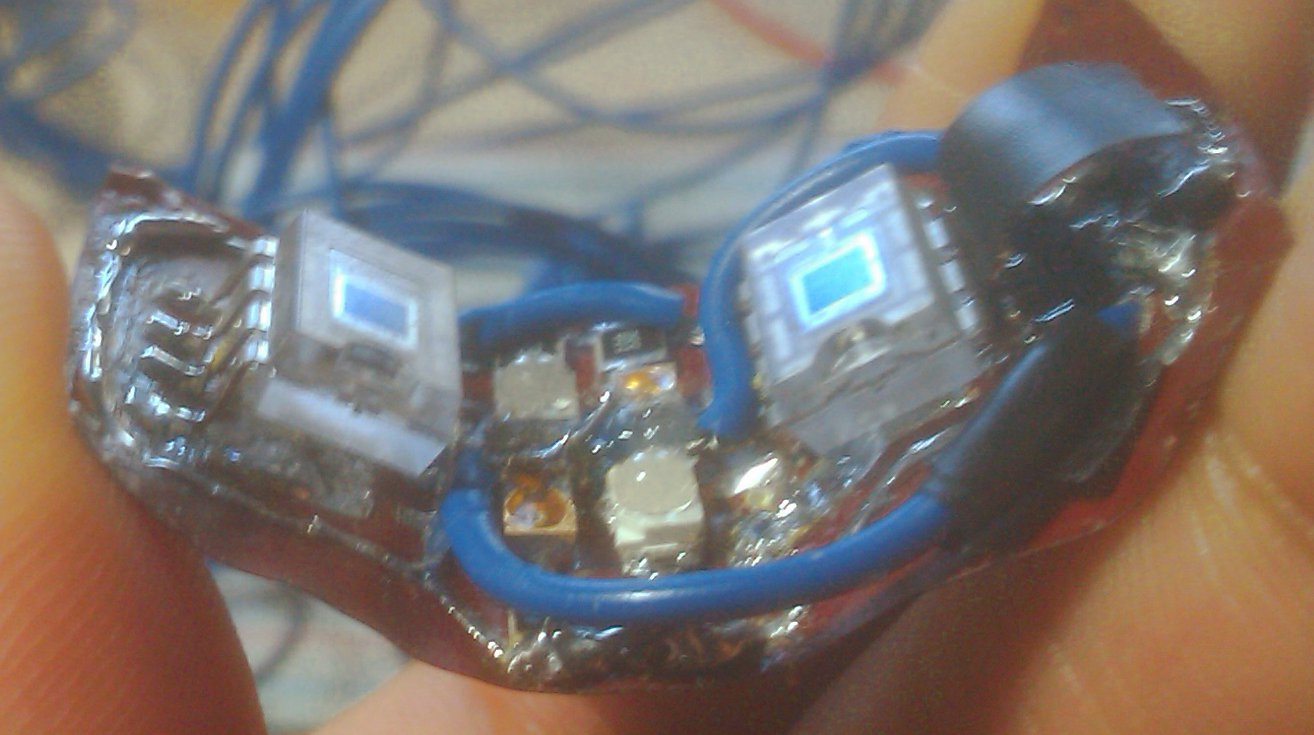
\includegraphics[width=6in]{csensorbend.jpg}}
\caption[Finalized Sensor Prototype]{The finalized complete sensor}
\end{figure}

\section{Software}

To write the software for the microcontroller, C was selected over assembly to reduce development time and increase readability. As discussed above, the UART function had to be written in software in addition to data acquisition. To do this, example timer UART code by L. Westlund at Texas Instruments, available in the IAR Embedded Workbench example files, was used as a basis for the software UART functionality. This was done because the author did not know how to implement the UART functionality from scratch. Once UART was working, data acquisition was tackled.

\subsection{Data Acquisition}
Due to the slow haemodynamic response in your brain due to activity, a time resolution of 10ms (or 100Hz) is all that is needed. That is all the wavelengths and positions must be sampled at least every 10 ms.

To do this, data is sampled in a time multiplexed fashion. That is, all the data is sampled independently in a certain order within the time resolution. 

Firstly the sensors are sampled with all the LEDs off to obtain the background light intensity. Then the first wavelength of LED is turned on and allowed to stabilize for a period of time. Then the first signal is obtained from the first OPT101 photodiode, subtracted by the background light intensity, and transmitted to the computer.  Then the second signal is obtained from the second OPT101 photodiode, subtracted by the background light intensity, and transmitted to the computer. Then the LEDs are turned off, the second wavelength LEDs turned on, allowed to stabilize, and the cycle repeated. Once this cycle is completed, all the LEDs are turned off, the background light intensity sampled, and the cycle repeats. This is illustrated in Figure 4.9. Though, perhaps it is more easily seen in the microcontroller code flow chart in Appendix B.1.

\begin{figure}[htp]
\centering
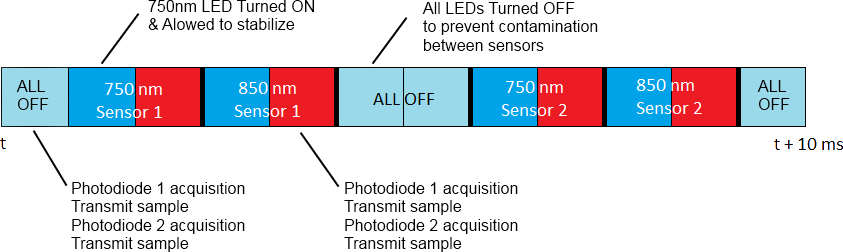
\includegraphics[width=6in]{data.png}
\caption[Time multiplexed acquisition]{An illustration of the time multiplexed acquisition cycle.}
\end{figure}

\subsection {Computer Software}

To write the software, Ruby was selected as the language of choice. It was selected due to the author's desire to learn Ruby as it is a very popular dynamic general purpose object-oriented programming language. It is spoken highly of by many experienced computer science veterans. While not up to the speed of C or C++, Ruby has amazingly good performance for a dynamic programming language.

The computer software must firstly obtain the data from the device. To do this the serialport library from rubygems (a host of many Ruby librarys or 'gems') was used to interact with the serial port on the computer, communicating through UART. The serial port is opened, sent the message 'S', to message the device to begin acquiring data. The program then receives the data. The data is split into two parts the upper 8 bit and the lower 8 bits when it is received. The program combines them together and divides the resulting value by 0xFFFF. The reason for this is the output from the ADC on the microcontroller is relative to its maximum value of 0xFFFF. To ensure the data arrives correctly, an 'S' is transmitted by the device before sending each set of data to ensure that the device is synchronized correctly with the computer. Once all the data is received, the calculations are done on the raw data to obtain the necessary relevant values.

Equations 3.7 and 3.8 were used to calculate the change in concentrations. Equation 3.6 was used to calculate the differential optical density. During the project demonstration Equation 3.6 was not written correctly in the code, giving wrong results. This has since been fixed and the differential optical density is now calculated correctly. In order to calculate the change in concentrations, first the specific wavelength constant and differential pathlength factors must be found.

Since the specific wavelength extinction coefficient of the absorber($\epsilon^\lambda$) cannot be directly measured with near infrared light, they are found by interpolating the values given for these coefficients for oxyhaemoglobin and deoxyhaemoglobin in literature, specifically \cite{wray88} and \cite{roe91}. This results in $\epsilon^{750nm}_Hb$ = 1.532, $\epsilon^{750nm}_O2Hb$ = 0.600, $\epsilon^{850nm}_Hb$ = 0.781, $\epsilon^{850nm}_O2Hb$ = 1.097. Calculating the differential pathlength factor (DPF$^\lambda$) yeilds $DPF^{730nm}$=5.0055 and $DPF^{850nm}$=4.6564. The calculation for DPF$^\lambda$ can be seen in Appendix A.2.

Once the calculations are complete the change in concentrations are output to text files that can be read by Matlab. The data is very noisy and requires a low pass filter to be done on it to obtain the necessary data. Due to time limitations, a low pass filter was not able to be made in Ruby for the software. As such, Matlab was decided to be used to filter the data. As per \cite{wolf05}, a low pass filter with a cutoff of 0.5Hz should be used. Therefore a low pass fourth-order butterworth filter was used with a cutoff of 0.5Hz. The Matlab source code can be seen in Appendix C. Taking the Fourier transform of the data before filtering gives the result in Figure 4.10(a). Taking the Fourier transform of the data after filtering gives the result in Figure 4.10(b).

\begin{figure}[htp]
\centering
\subfigure[FFT of data before filtering]{ 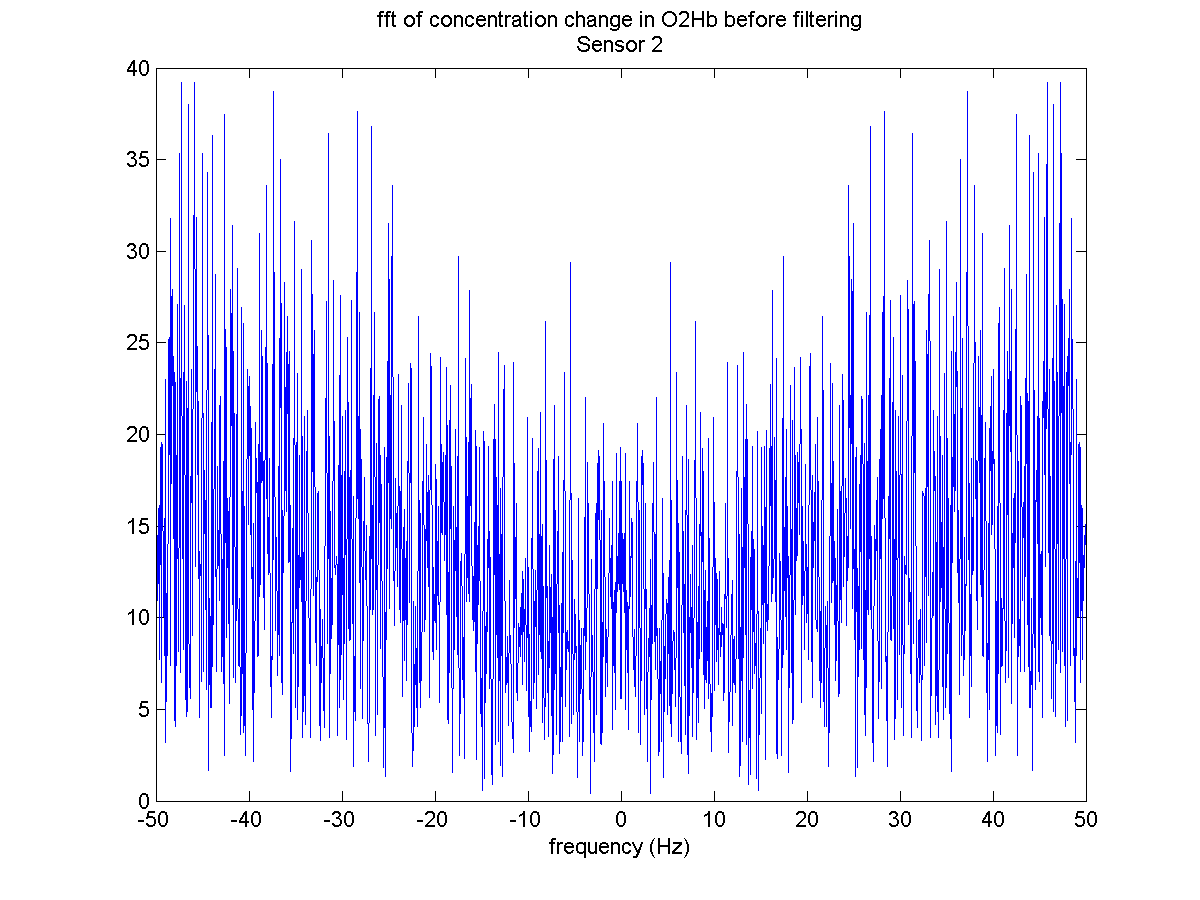
\includegraphics[width=4in]{fftHbO2_2.png}}
\subfigure[FFT of data after filtering]{ 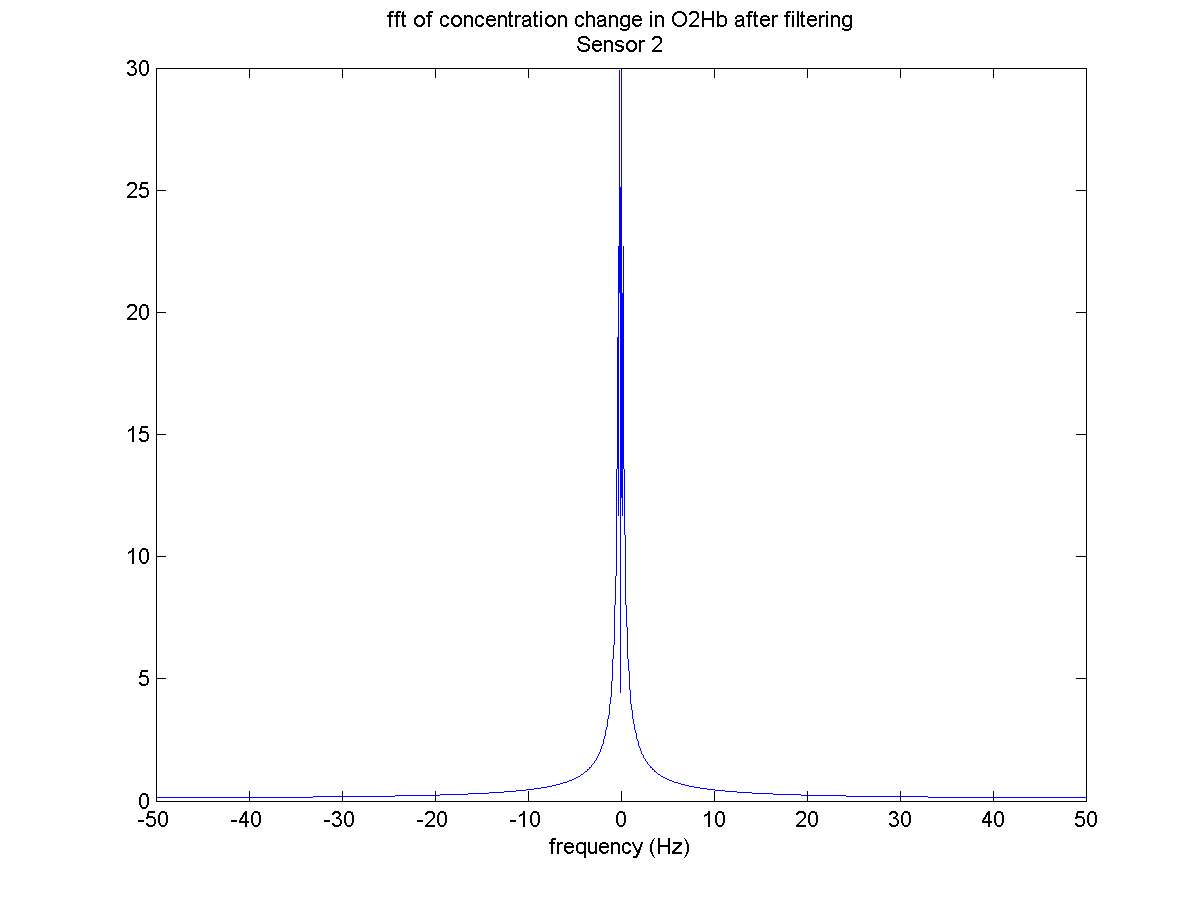
\includegraphics[width=4in]{fftHbO2_2f.png}}
\caption[FFT of data]{The FFT of the data before filtering and after filtering. The data used is the change in oxyhaemoglobin during motor movement}
\end{figure}

The design of the device is now complete and results can be seen.

\section{Cost}

Since one of the goals of this project is to low-cost, Table 4.1 shows the total cost to build one of these systems with one sensor. The USB to UART module will be left out since it is only needed for programming the device. In a mass produced system, the microcontroller would be programmed by JTAG anyway.

\begin{table}
  \caption{Cost of 1 NIRS System}
  \begin{tabular}{| l | c | r | r |}
\hline
\multicolumn{4}{|c|}{Cost of 1 NIRS System} \\
\hline
\bf Item & \bf Quantity & \bf Unit Price & \bf Total Price \\ \hline
LDO Regulator&1&\$1.85&\$1.85\\
1$\mu$f Capacitors&4&\$0.05&\$0.20\\
0.01$\mu$f Capacitors&4&\$0.01&\$0.04\\
32KHz Crystal&1&\$0.36&\$0.36\\
MSP430f4250&1&\$4.55&\$4.55\\
Power LED&1&\$0.10&\$0.10\\
330$\Omega$ Resistor&2&\$0.06&\$0.12\\
Bluetooth LED&1&\$0.12&\$0.12\\
Bluetooth module&1&\$18.00&\$18.00\\
SPDT Switch&1&\$3.99&\$3.99\\
2N4401 BJT&2&\$0.14&\$0.28\\ \hline
\multicolumn{3}{|r}{\em Subtotal}&\$29.61 \\ \hline
\multicolumn{4}{|l|}{\bf Sensor} \\ \hline
750nm LED&2&\$3.02&6.04\\
850nm LED&2&\$1.17&\$2.34\\
33$\Omega$ Resistor&4&\$0.17&\$0.68\\
OPT101 Photodiode&2&\$6.23&\$12.46\\ \hline
\multicolumn{3}{|r}{\em Subtotal}&\$21.52 \\ 
\multicolumn{3}{|r}{\bf \em Total}&\bf \$51.13 \\
\hline
  \end{tabular}
\end{table}

\section{Design Challenges}
The initial design challenges encountered were sourcing the LEDs. A consumer retailer could not be found selling LEDs of a wavelength between 700nm - 830nm. Many email had to be sent out to various manufacturers, retailers, and distributors until the Marubeni Corporation responded that they would be willing to sell some samples.

The Majority of the other design challenges stem from the author's inexperience with microcontroller design and time constraints. 

Perhaps one of the longest challenges that had to be overcome was the UART communication. After the prototype was built, it would not communicate over UART via the USB to UART module. After much troubleshooting and going over the design many times, comparing my circuit design to another MSP430 project that used UART, it was determined that the TX and RX wires were swapped. Originally the TX output from the USB UART module was connected to the TX output of the microcontroller and the RX input connected to the RX input. Due to inexperience, the author believed that the connection matched up rather than the logical way of TX to RX.

Now that the bootloader was able to be programmed, implementing the software timer UART was a daunting task. Writing custom code proved to be futile, so example code was turned to for the UART implementation. However, even unmodified sample code was not communicating to the computer. Code was executing correctly on the device, it was possible to to flash LEDs and such. However, once a serial terminal was opened on the computer, code would stop executing, as if it was stuck in an interrupt. Due to the decision to not use a JTAG programmer, debugging could only be done via LEDs. 

After many countless hours, it was realized that the DTR line on the USB UART module was setting RST to low on the microcontroller, resetting the device. The RST wire is there because it is needed to invoke the bootloader and is part of the flow control used by the built-in bootloader. However, it must be disconnected when not trying to invoke the bootloader.

The flexible sensor provided a great design challenge. If the  creation of the sensor was not difficult enough, populating the board was. Due to the decision to make the sensor as small as possible and being only a single sided SMD PCB, jumper wires were used to connect certain components. This made it a large pain to solder the components. Additionally, small traces were selected. Had the board been ridged rather than flexible, this design would have been fine since the traces came out okay. But after many bends and flexes, some of the traces broke, even if they appeared to be okay. These were easily fixable by soldering the traces back together. However, it provided a big headache when testing the device.

The computer software also played a somewhat large challenge and is perhaps the weakest part of this project and the main reason for its poor performance. Data acquisition played a problem at first. The microcontroller and computer were not in sync, and the computer received many null data points when trying to retrieve the data. However after properly matching the times between the two programs through the use of sleep functions, the data was retrieved correctly. The switch to the Bluetooth module removed these errors, everything synced up fine and the sleep functions code be removed. It is assumed that there are performance issues with the FTDI USB UART driver in Linux. However, the microcontroller still sends the char 'S' before each measurement to ensure everything syncs up fine.                  % the first chapter
        \setcounter{figure}{0}
        \setcounter{equation}{0}
        \setcounter{table}{0}

  \chapter{Results and Discussion}

\section{Motor Movement}
Due to the high objectivity of brain activity due to motor movement, measuring brain activity due to motor movement is perhaps the best way to asses the system. Placing the sensor above the top left motor cortex (refer to Figure 5.1), and having the test subject do the 'chicken dance' (that is repeatably touching the thumb to the tip of each finger) with their right hand for 30s yields the results in Figure 5.2. Note that the subject started the 'chicken dance' at around 1s, stopped movement to see the effect, then resumed the chicken dance again, and then finally stopped movement before the end of the test.

\begin{figure}[htp]
\centering
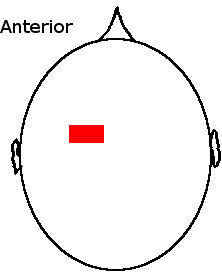
\includegraphics[width=2in]{motorsens.png}
\caption[Placement of Sensor to Measure Right Hand Movement]{Approximate placement of the sensor to measure right hand movement. The sensor, marked in red, is positioned above the left motor cortex.}
\end{figure}

\begin{figure}[htp]
\centering
\subfigure[Sensor 1]{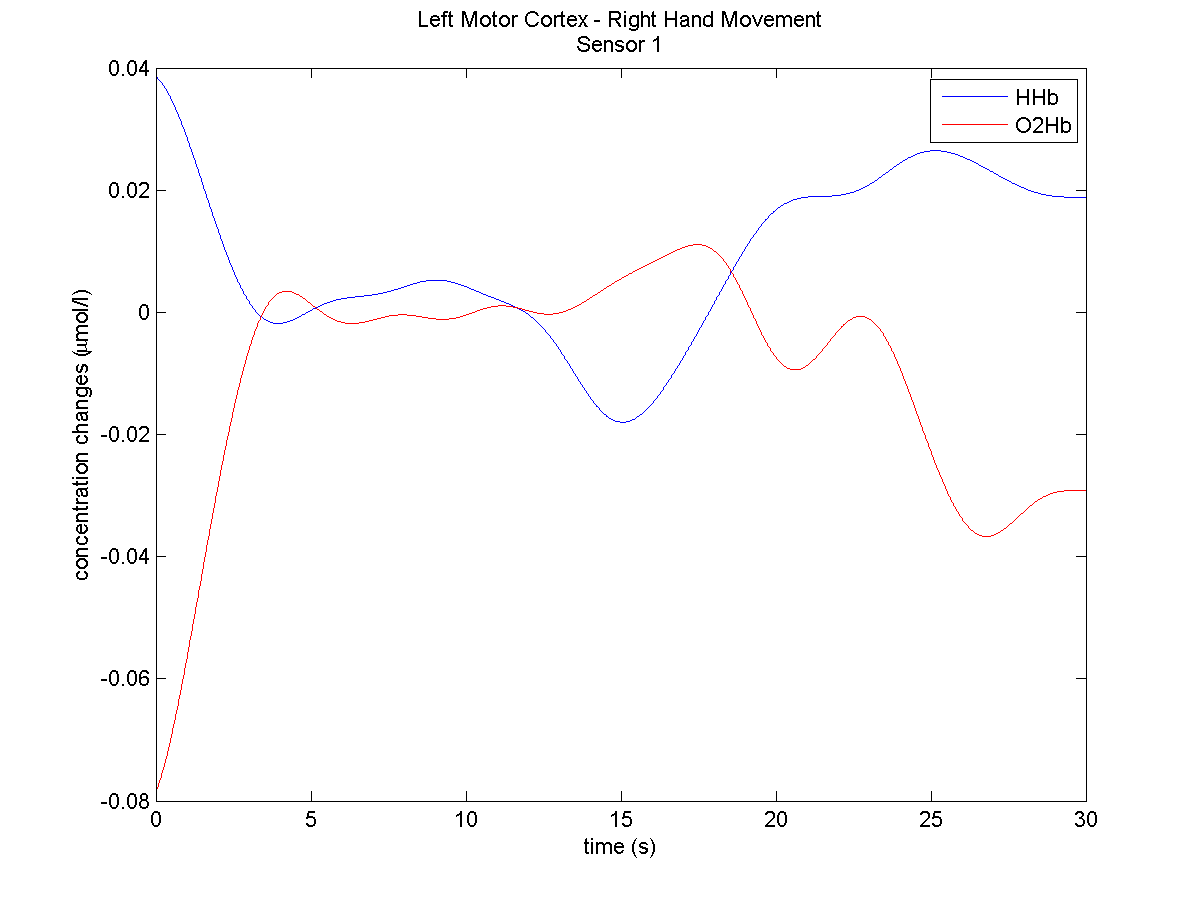
\includegraphics[width=4in]{LeftMotorCortex-RightHandMovement/sensor1.png}}
\subfigure[Sensor 2]{ 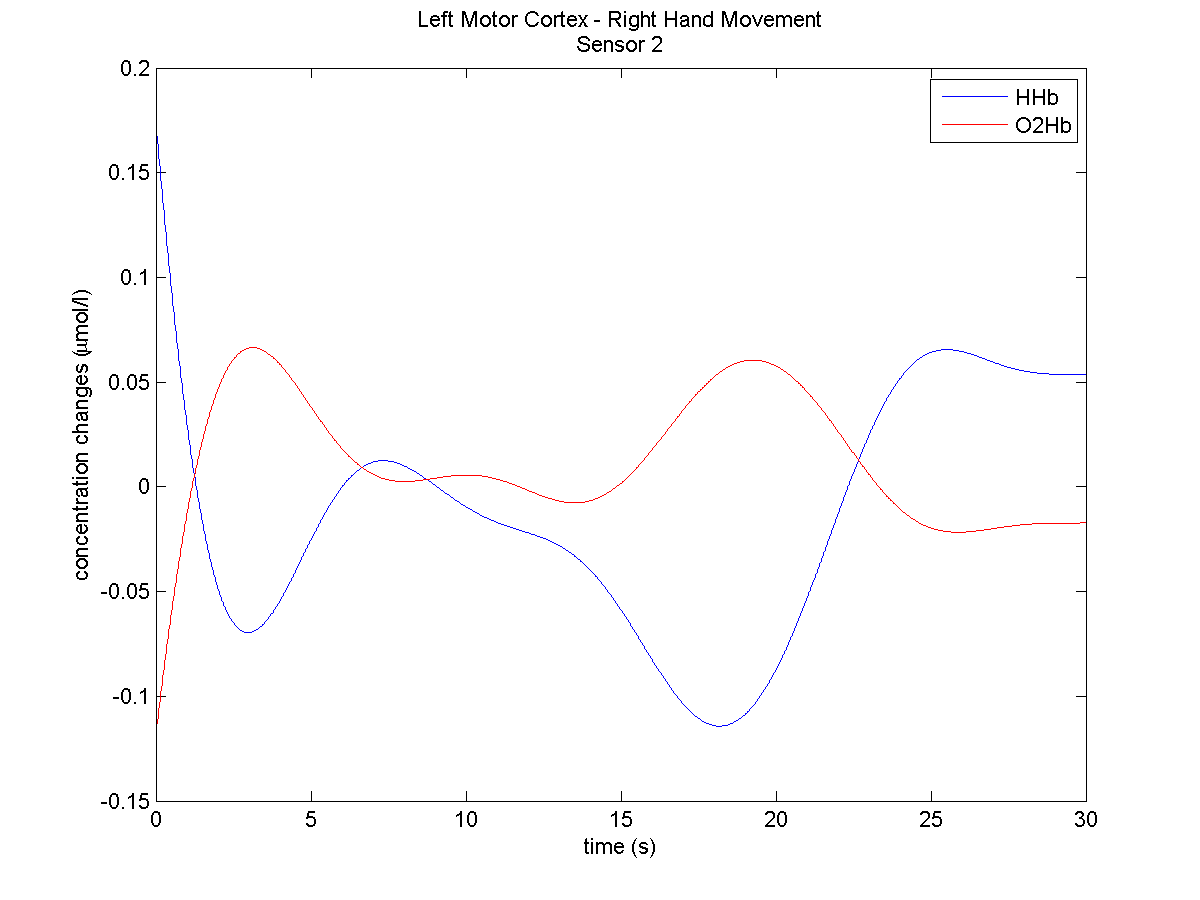
\includegraphics[width=4in]{LeftMotorCortex-RightHandMovement/sensor2.png}}
\caption[Left Motor Cortex Measurements with Motor Movement]{The result of having the subject move their right hand with the sensor placed over the left motor cortex. The change in concentration of oxyhaemoglobin is marked in red and the change in concentration of deoxyhaemoglobin is marked in blue. The subject began the 'chicken dance' at ~1s, briefly stopped at around 7s, started the 'chicken dance' again at around 9s, and finally stopped at around 22s, as can be seen in the Sensor 2 measurements.}
\end{figure}

The measurements from Sensor 1 do not seem to be correct. It is excessively noisy, masking the haemodynamic effect of the blood perfusion that is the result of the motor movement. Perhaps, the photodiode is damaged or the lens scratched/dirty. There was not enough time to correctly trouble shoot the problem. In either case, the results from Sensor1, while it does pick up varying light intensities, contains too much noise to extract the relevant data from it. As such, the results from Sensor 1 should be ignored. However, for the sake of completeness and to correctly asses the system, figures of the measurements from Sensor 1 will still be included, though not discussed. 

Looking at the figures, it can be seen that the concentration changes at the start of the measurements, while relevant, are much larger compared to the rest. This is a result of initially measuring the system from 0, thus there is a high concentration change from the beginning. Once the correct base level is achieved, the results normalize and the exact concentration changes can be seen. Therefore, when looking at the results one can safely ignore the first few measurements. One thing to note about these measurements is that the subject had long dark hair, which will decrease the overall SNR of the system.

Analyzing at the results from Sensor 2, it can be seen that with motor activity on the right part of the body, there is an increased amount of oxyhaemoglobin concentration and a decreased amount of deoxyhaemoglobin concentration. When motor activity stops (at around 7s), the amount of oxyhaemoglobin concentration decreases and the amount of deoxyhaemoglobin concentration increases. When motor activity starts up again (at around 9s), again there is an increased amount of oxyhaemoglobin concentration and a decreased amount of deoxyhaemoglobin concentration. When the motor activity finally stops completely, the amount of oxyhaemoglobin concentration decreases and the amount of deoxyhaemoglobin concentration greatly increases. This agrees with what one would expected from neuronal activation. With neuronal activation comes an increased amount of blood perfusion, thus increased amounts of oxyhaemoglobin and decreased amount of deoxyhaemoglobin. When neuronal activation stops, blood perfusion decreases, adversely, causing decreased amounts of oxyhaemoglobin and increased amount of deoxyhaemoglobin. This also agrees with the results obtained from other NIRS systems (refer to Chapter 2, Figures 2.2 and 2.3 specifically).

To better analyze motor movement, lets have a look at the same measurements but with no motor movement. To examine the case with no motor movement, the sensor was placed in roughly the same place as in Figure 5.1 with the subject attempting to stay perfectly still. The results of this are displayed in Figure 5.3.

\begin{figure}[htp]
\centering
\subfigure[Sensor 1]{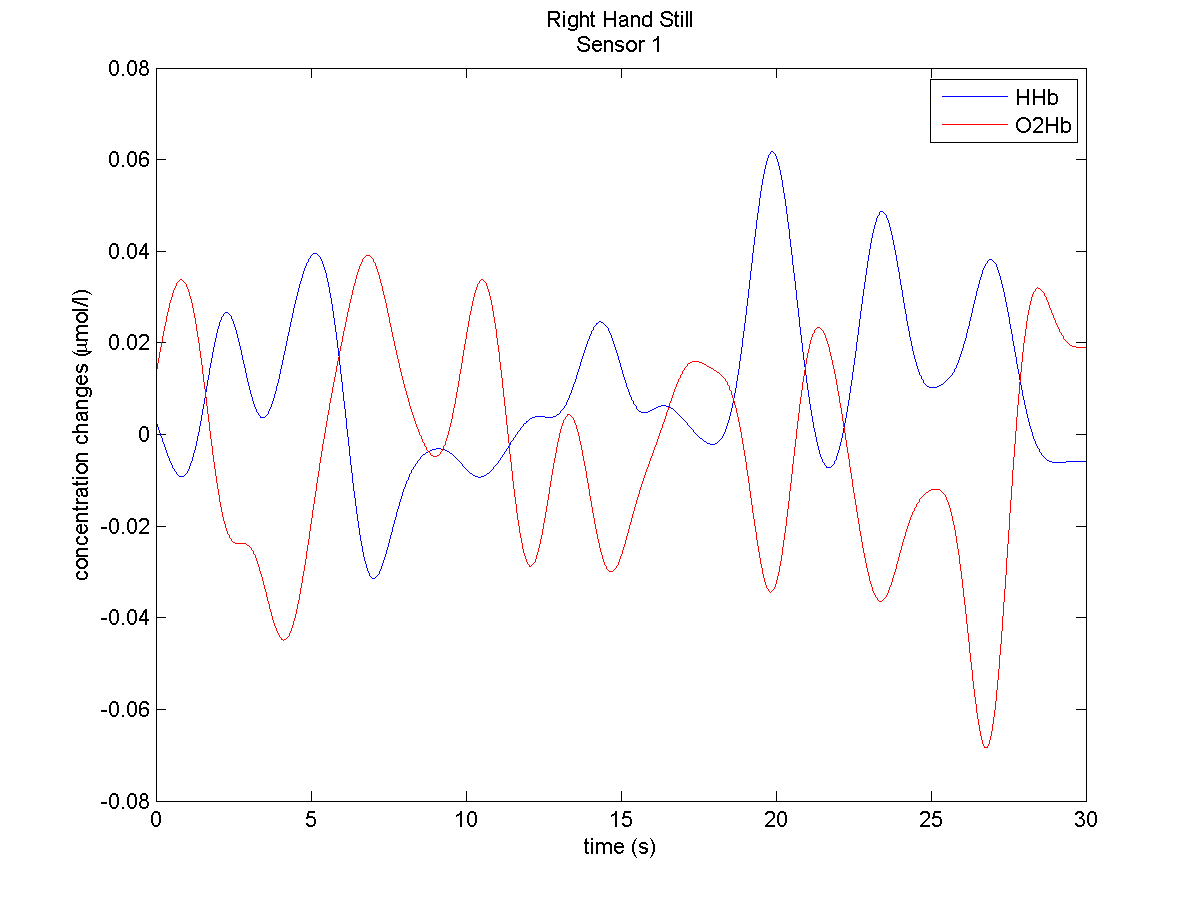
\includegraphics[width=4in]{LeftMotorCortex-NoMovement/sensor1.png}}
\subfigure[Sensor 2]{ 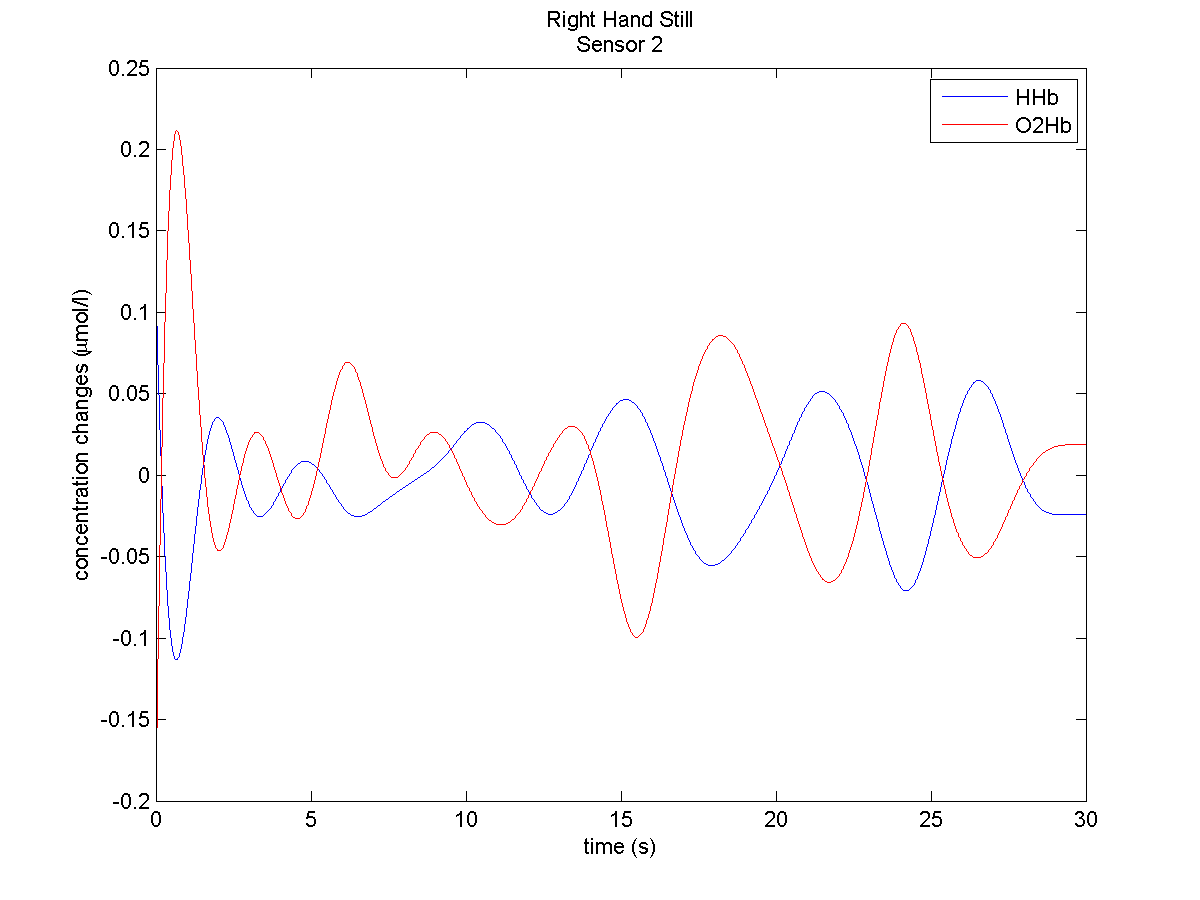
\includegraphics[width=4in]{LeftMotorCortex-NoMovement/sensor2.png}}
\caption[Left Motor Cortex Measurements with No Motor Movement]{The result of having the subject attempt to sit still with the sensor placed over the left motor cortex. The change in concentration of oxyhaemoglobin is marked in red and the change in concentration of deoxyhaemoglobin is marked in blue.}
\end{figure}

The results in Figure 5.3 show that when the subject is at rest, there is no constant increase or decrease in oxyhaemoglobin or deoxyhaemoglobin. Rather, the change in concentration constantly increases and decreases. This is probably caused by cells in the neuron consuming oxygen, increasing the deoxyhaemoglobin concentration, but with the increased level of deoxyhaemoglobin, fresh blood enters the neuron, increasing the oxyhaemoglobin concentration. With this cycle repeating itself, the results obtained would mirror that of in Figure 5.3.

To test the repeatably of this NIRS device, the same motor movement ('the chicken dance') will be done again with the sensor in roughly the same place as in Figure 5.1. It can be seen in Figure 5.4.

\begin{figure}[htp]
\centering
\subfigure[Sensor 1]{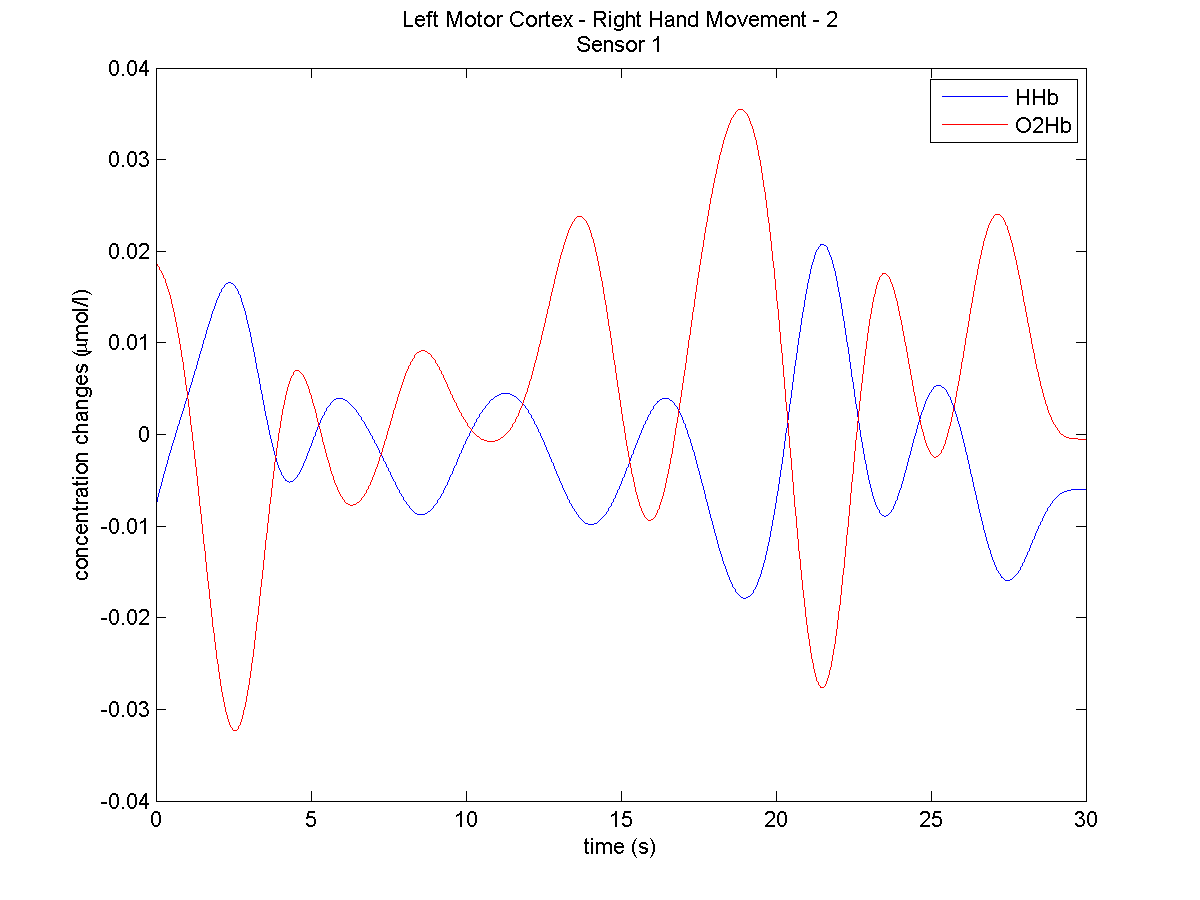
\includegraphics[width=4in]{LeftMotorCortex-RightHandMovement-2/sensor1.png}}
\subfigure[Sensor 2]{ 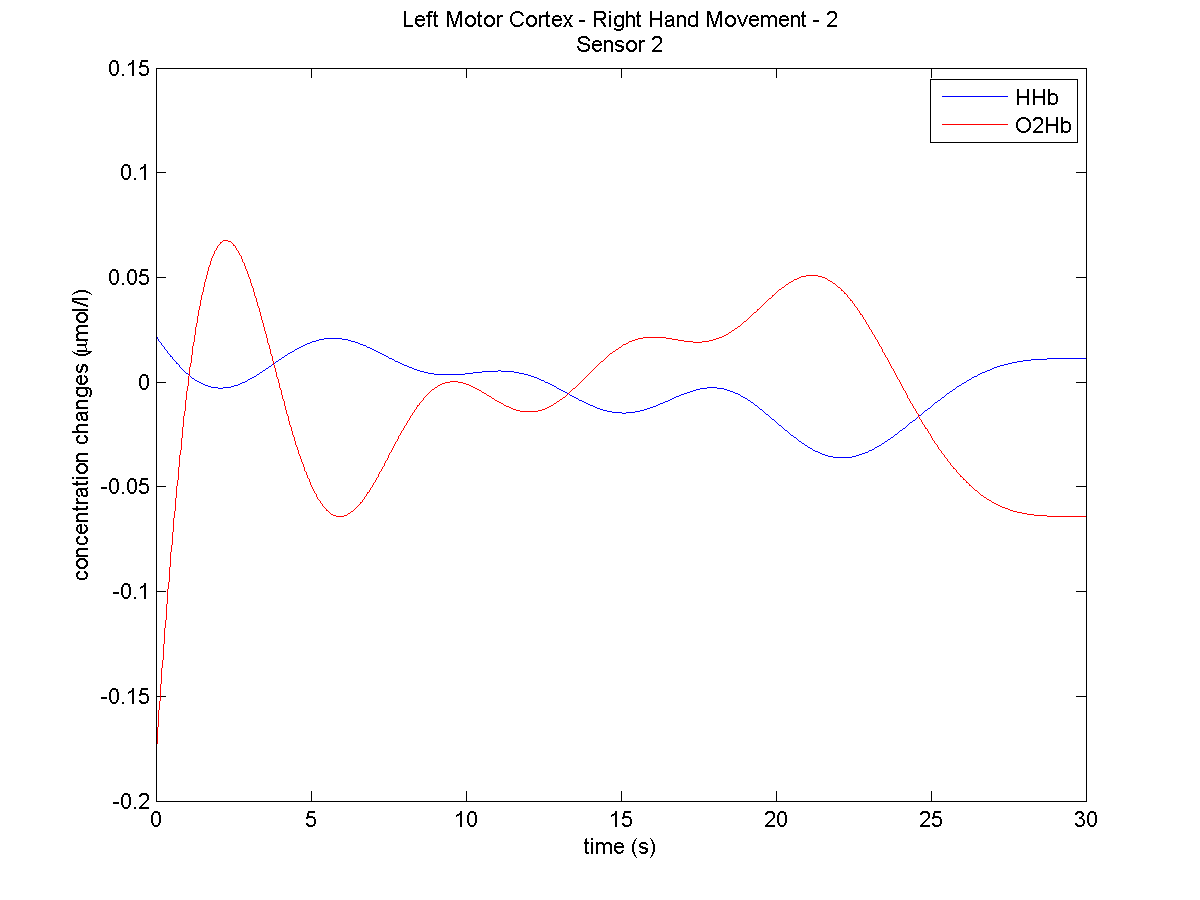
\includegraphics[width=4in]{LeftMotorCortex-RightHandMovement-2/sensor2.png}}
\caption[Left Motor Cortex Measurements with Motor Movement, Test 2]{The second result of having the subject do the 'chicken dance' with their right hand with the sensor placed over the left motor cortex. The change in concentration of oxyhaemoglobin is marked in red and the change in concentration of deoxyhaemoglobin is marked in blue. This time the subject began movement at around 0s, stopped at around 4s, and slowly began the 'chicken dance' again at around 8s before finally stopping at roughly 25s.}
\end{figure}

The results in Figure 5.4 show a good amount of repeatability. The results agree with that in the first test of right hand motor activity. When there is motor activity on the right part of the body, there is an increased amount of oxyhaemoglobin concentration and a decreased amount of deoxyhaemoglobin concentration. When the motor activity stops, the amount of oxyhaemoglobin concentration decreases and the amount of deoxyhaemoglobin concentration increases.

Doing the same test with the left hand and the sensor placed on top of the right motor cortex (refer to Figure 5.5) gives the results in Figure 5.6.

\begin{figure}[htp]
\centering
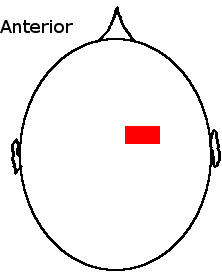
\includegraphics[width=2in]{motorsens-left.png}
\caption[Placement of Sensor to Measure Left Hand Movement]{Approximate placement of the sensor to measure left hand movement. The sensor, marked in red, is positioned above the right motor cortex.}
\end{figure}

\begin{figure}[htp]
\centering
\subfigure[Sensor 1]{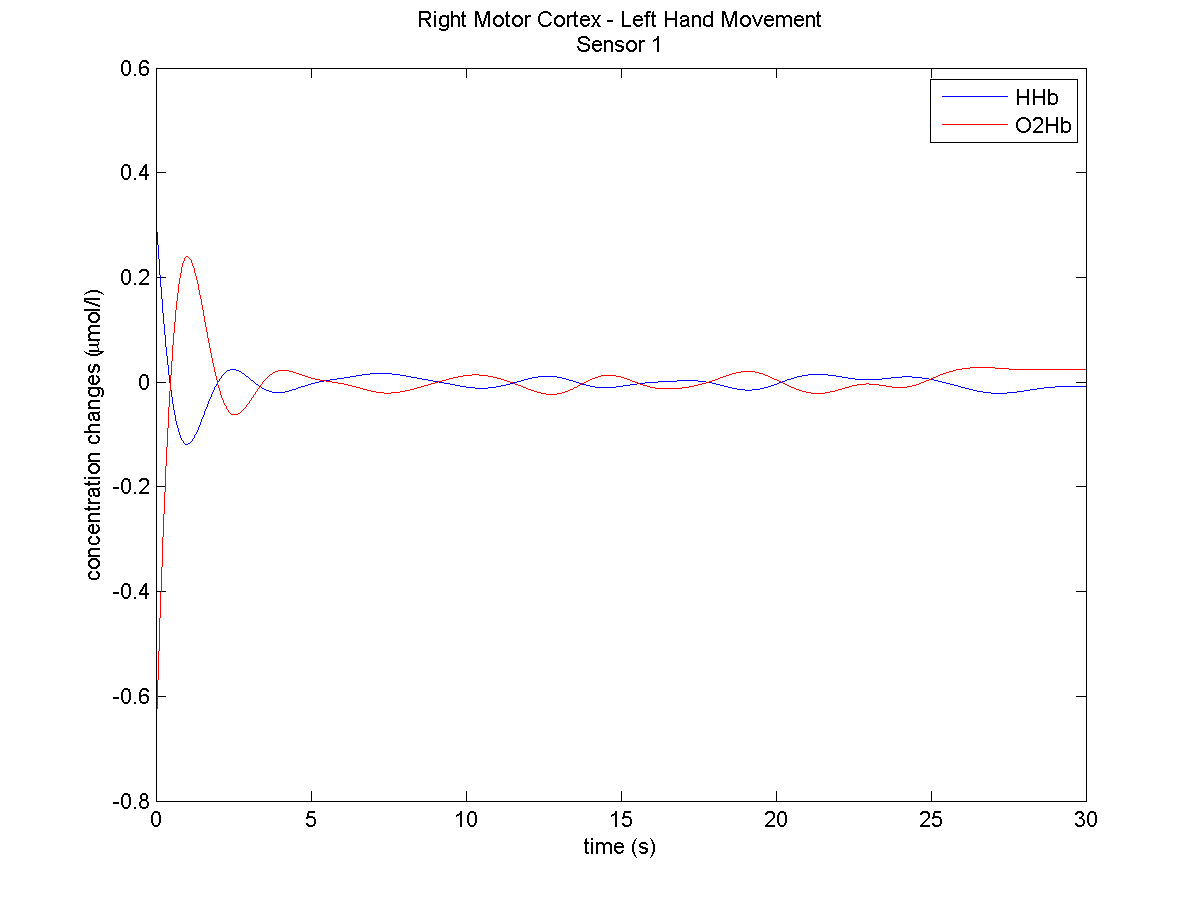
\includegraphics[width=4in]{RightMotorCortex-LeftHandMovement/sensor1.png}}
\subfigure[Sensor 2]{ 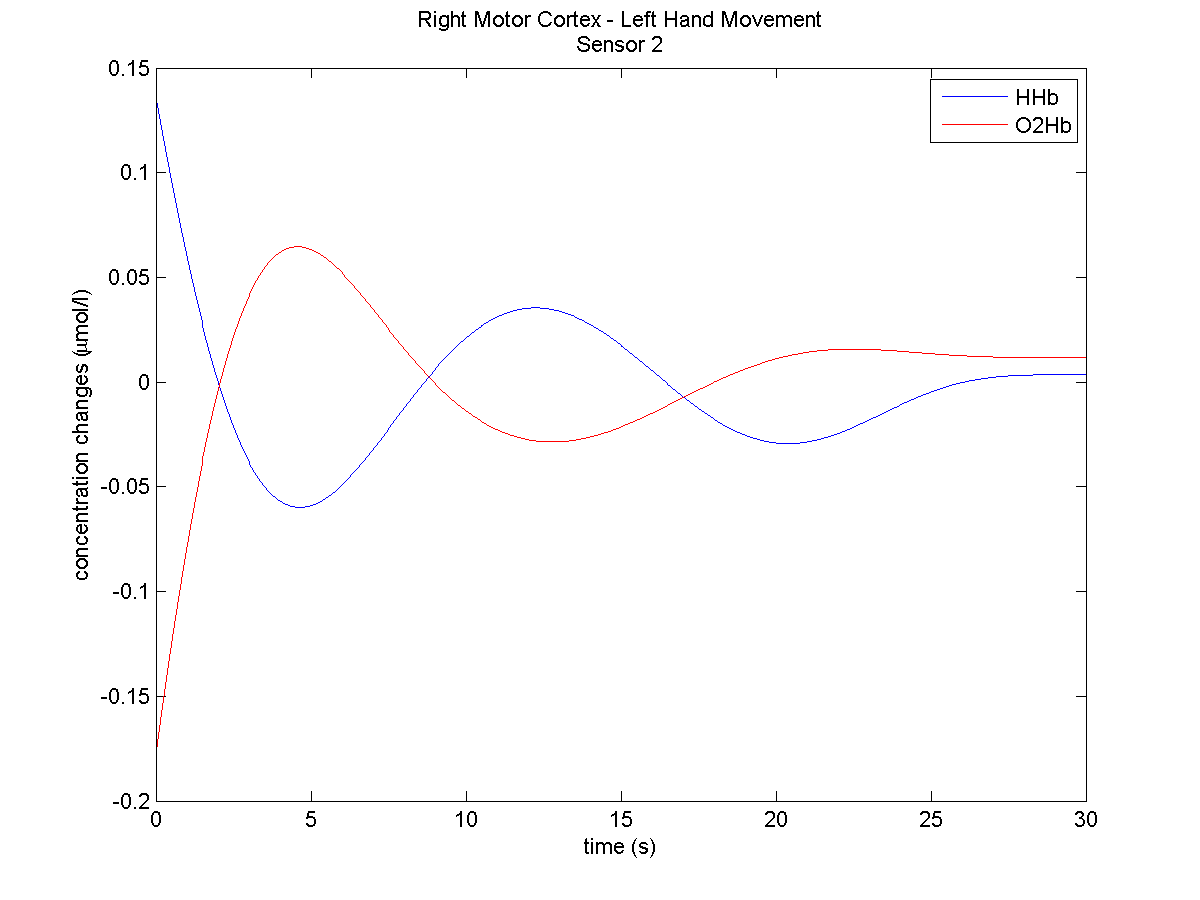
\includegraphics[width=4in]{RightMotorCortex-LeftHandMovement/sensor2.png}}
\caption[Left Motor Cortex Measurements with Motor Movement]{The result of having the subject move their left hand with the sensor placed over the right motor cortex. The change in concentration of oxyhaemoglobin is marked in red and the change in concentration of deoxyhaemoglobin is marked in blue. The subject began the 'chicken dance' at ~0s, stopped at around 7s, and started the 'chicken dance' again at around 16s, as can be seen in the Sensor 2 measurements.}
\end{figure}

Once again, it can be seen that with motor activity on the left part of the body, there is an increased amount of oxyhaemoglobin concentration and a decreased amount of deoxyhaemoglobin concentration in the right side of the motor cortex. Once more, when motor activity stops, the amount of oxyhaemoglobin concentration decreases and the amount of deoxyhaemoglobin concentration increases.

\section{Thinking Intensely}
Now that it has been shown that the NIRS device can somewhat accurately measure brain activity, others areas of the brain can be explored. Measuring brain activity in the frontal lobe while thinking about random things can be done when the sensor is placed as seen in Figure 5.7. This yields the results in Figure 5.8. Doing the same measurements but with the subject's eyes closed and in a relaxed state with the subject trying not to think about anything yields the results in Figure 5.9.

\begin{figure}[htp]
\centering
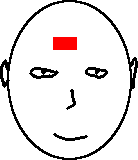
\includegraphics[width=2in]{sensorfront.png}
\caption[Placement of Sensor to measure Frontal Lobe]{Approximate placement of the sensor to measure brain activity when thinking intently. The sensor, marked in red, is positioned above the frontal lobe.}
\end{figure}

\begin{figure}[htp]
\centering
\subfigure[Sensor 1]{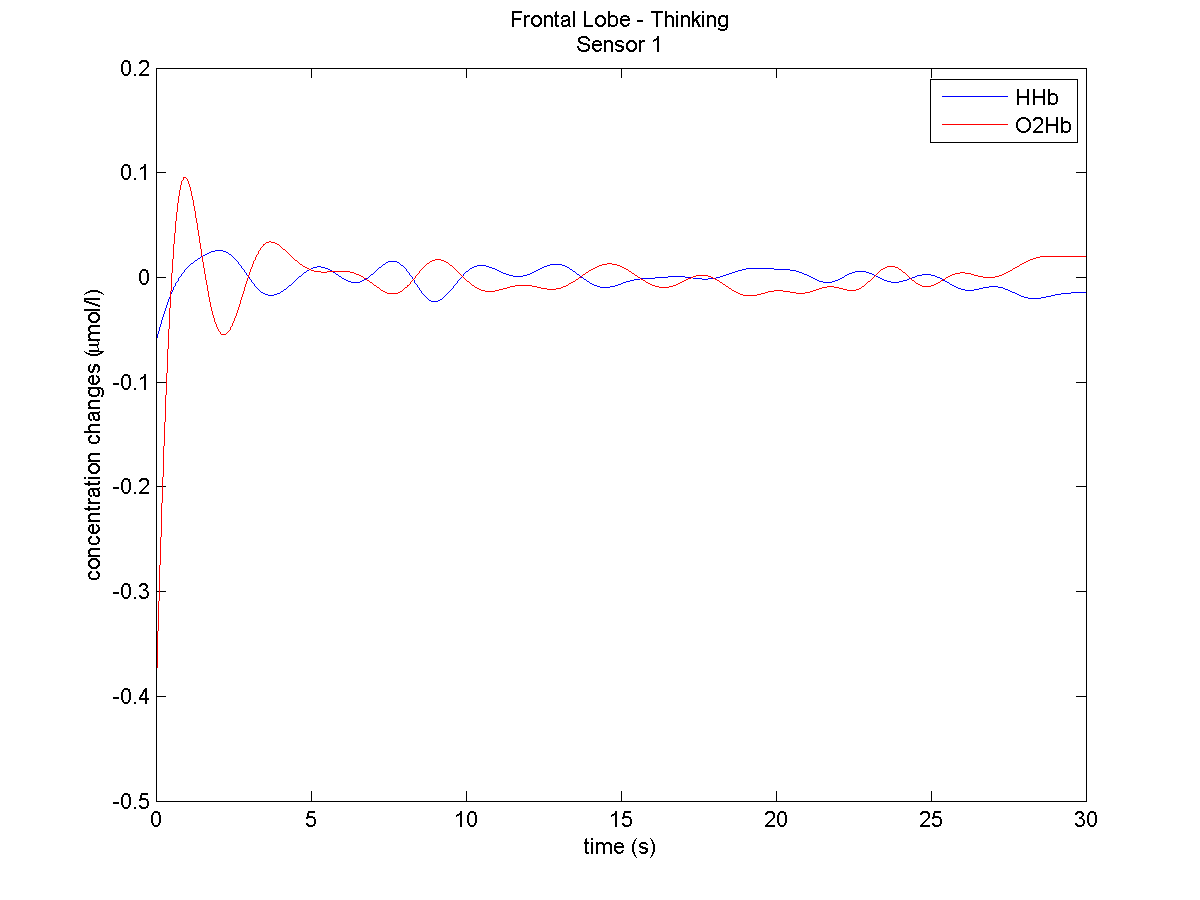
\includegraphics[width=4in]{FrontalLobe-Thinking/sensor1.png}}
\subfigure[Sensor 2]{ 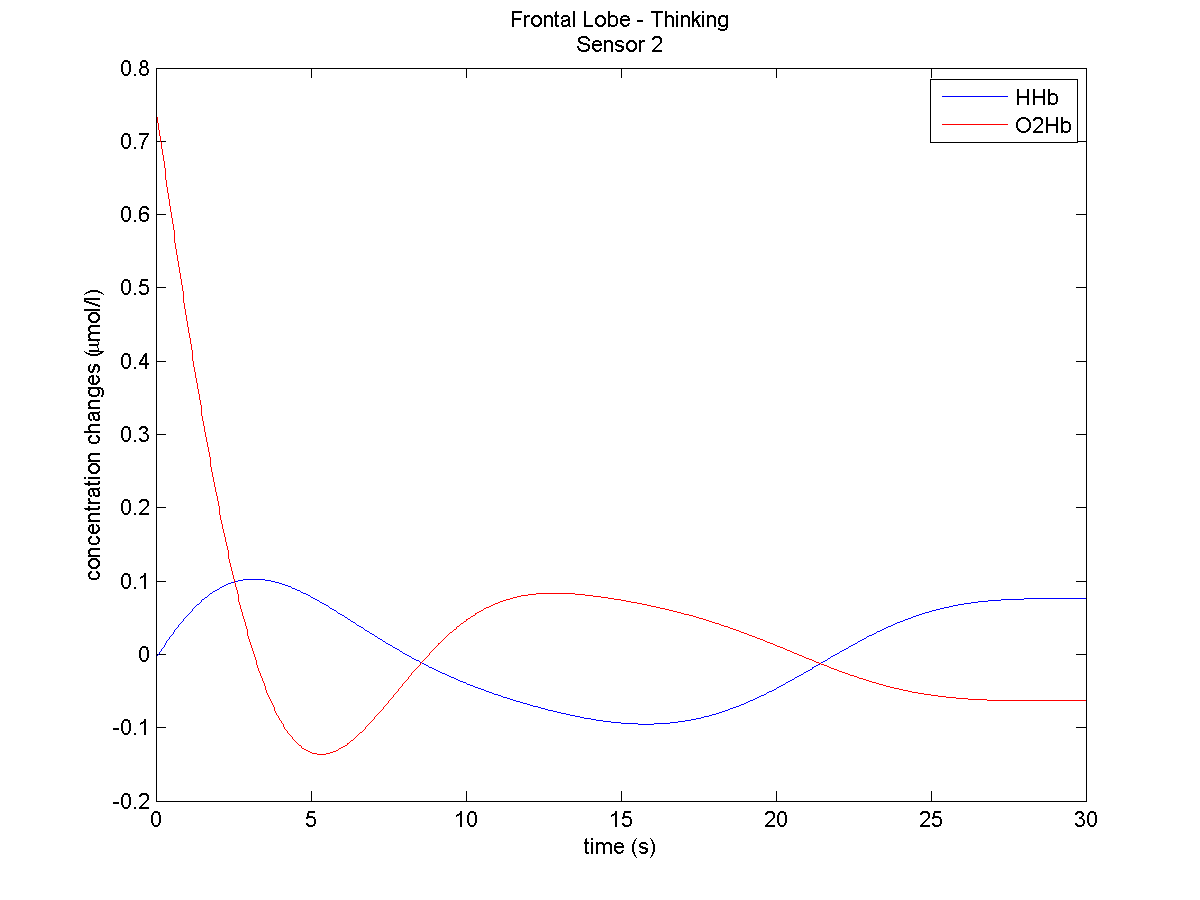
\includegraphics[width=4in]{FrontalLobe-Thinking/sensor2.png}}
\caption[Frontal Lobe Measurements while Thinking Intensely]{The result of having the subject think intensely with the sensor placed over the frontal lobe. The change in concentration of oxyhaemoglobin is marked in red and the change in concentration of deoxyhaemoglobin is marked in blue.}
\end{figure}

\begin{figure}[htp]
\centering
\subfigure[Sensor 1]{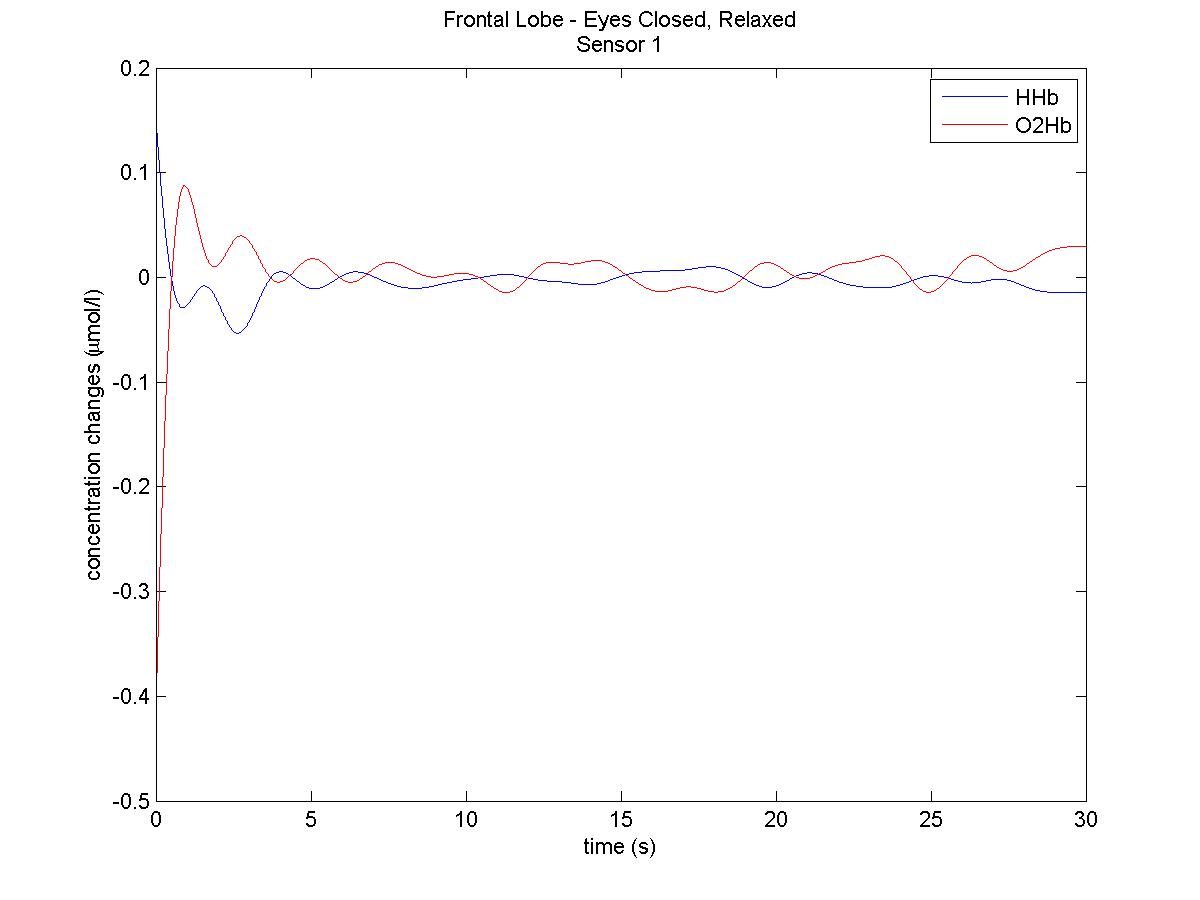
\includegraphics[width=4in]{FrontalLobe-Relaxed/sensor1.png}}
\subfigure[Sensor 2]{ 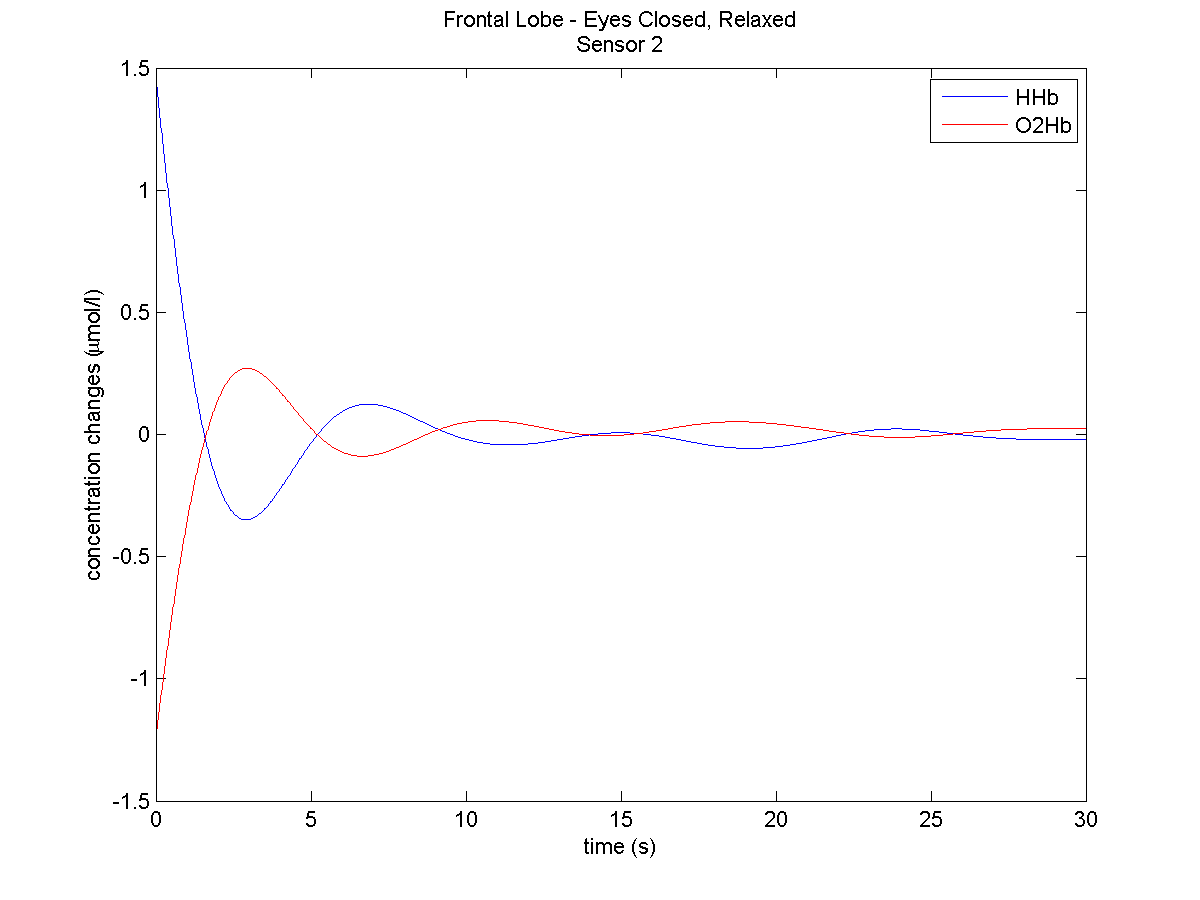
\includegraphics[width=4in]{FrontalLobe-Relaxed/sensor2.png}}
\caption[Frontal Lobe Measurements while Relaxed]{The result of having the subject not think of anything in a relaxed manor and their eyes closed with the sensor placed over the frontal lobe. The change in concentration of oxyhaemoglobin is marked in red and the change in concentration of deoxyhaemoglobin is marked in blue.}
\end{figure}

Comparing the 2 results, it can be seen that brain activity while the subject is thinking intensely can indeed by measured. When the subject is thinking intensely there is a constant increase in oxyhaemoglobin and constant decrease in deoxyhaemoglobin, showing brain activity. However, when the subject is in a relaxed non-thinking manor, the change in concentrations of oxyhaemoglobin and deoxyhaemoglobin constantly fluctuate; they are continually increases and decreasing.

\section{Visual stimulation}
Measuring the visual cortex with the subject's eyes continually moving from one intensely focused object to another, gives the results in Figure 5.11. The sensor placement can be seen in Figure 5.10. Doing the same measurements but with the subject's eye's closed, produces the result in Figure 5.12.

\begin{figure}[htp]
\centering
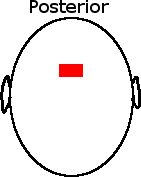
\includegraphics[width=2in]{sensorback.png}
\caption[Placement of Sensor to Measure Visual Cortex]{Approximate placement of the sensor to measure brain activity in the visual cortex. The sensor, marked in red, is positioned on top of the visual cortex.}
\end{figure}

\begin{figure}[htp]
\centering
\subfigure[Sensor 1]{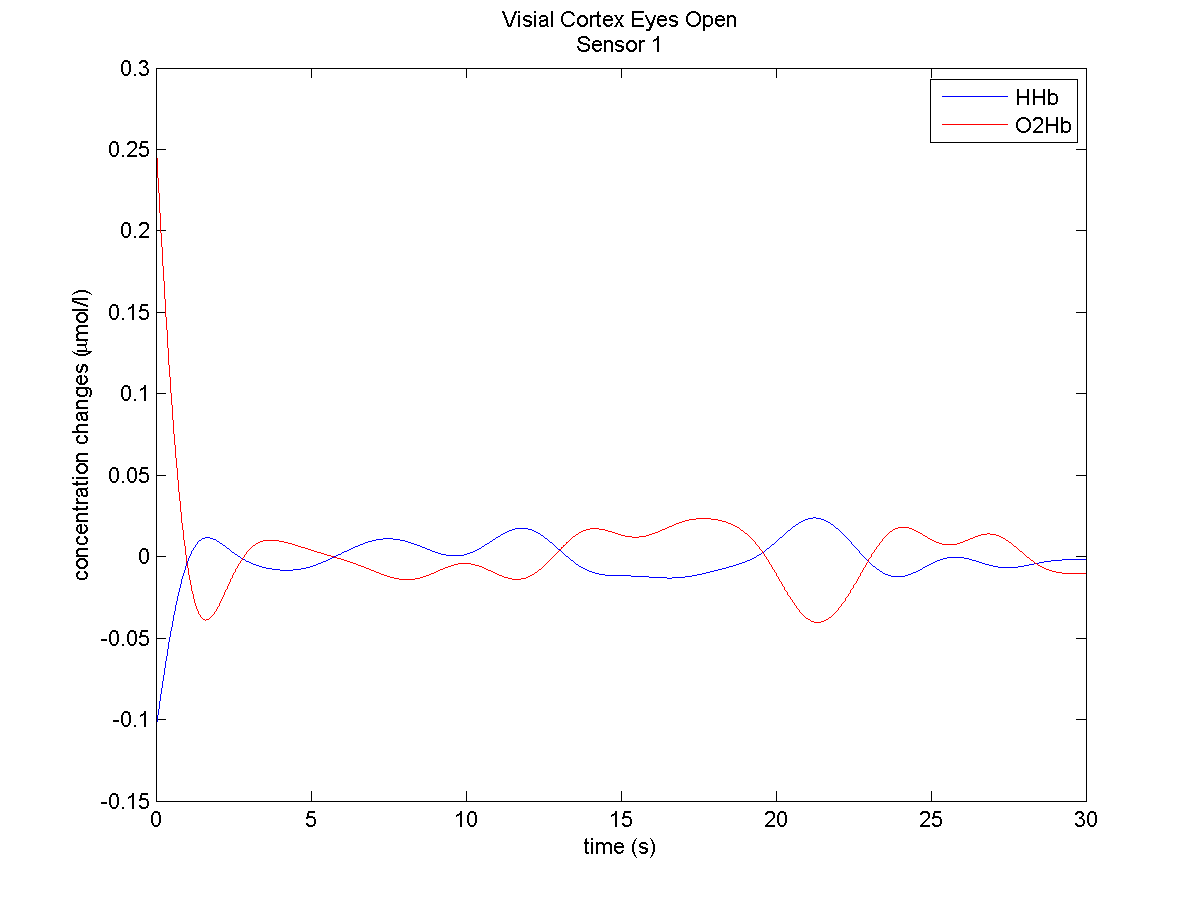
\includegraphics[width=4in]{VisialCortex-EyesOpen/sensor1.png}}
\subfigure[Sensor 2]{ 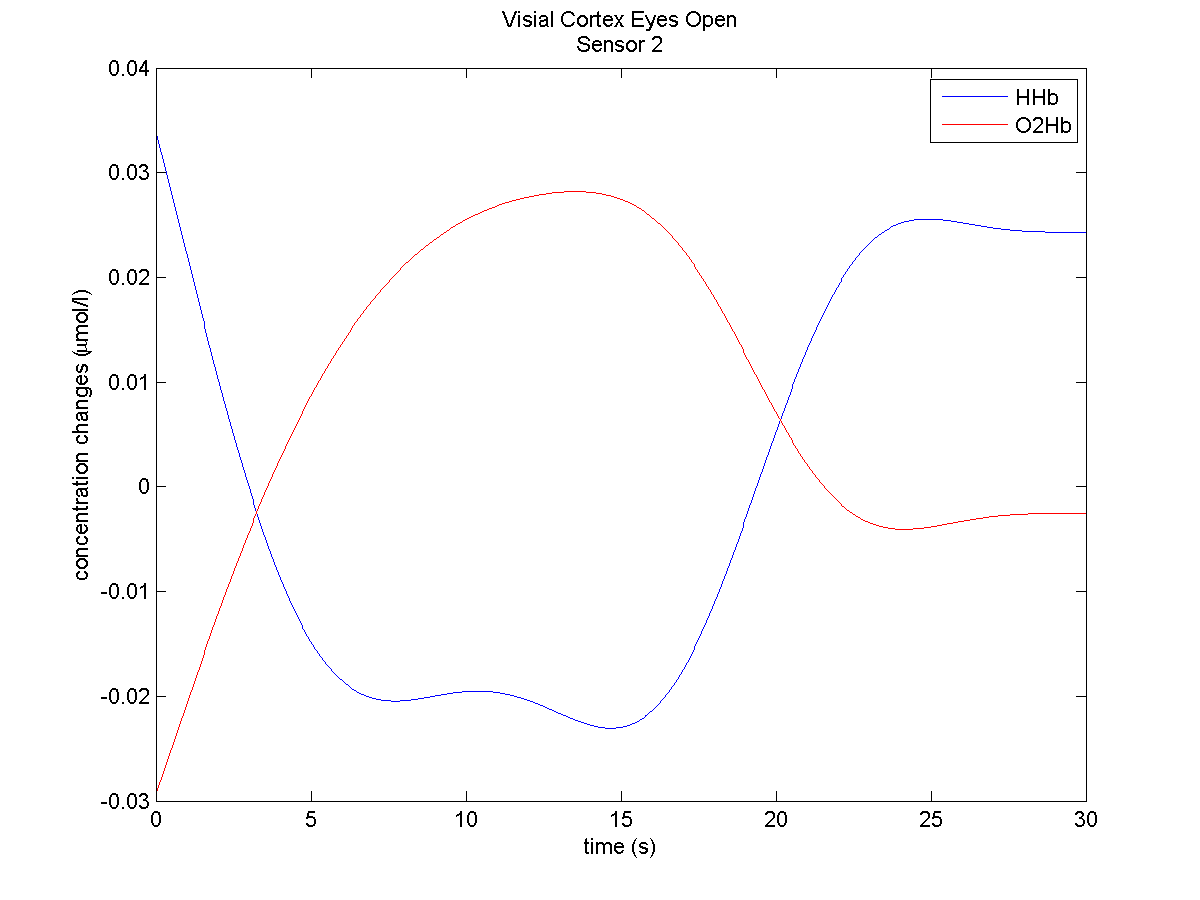
\includegraphics[width=4in]{VisialCortex-EyesOpen/sensor2.png}}
\caption[Visual Cortex Measurements while Moving Eyes between focused objects]{The result of having the subject constantly moving their eyes from different intensely focused object with the sensor placed over the visual cortex. The change in concentration of oxyhaemoglobin is marked in red and the change in concentration of deoxyhaemoglobin is marked in blue.}
\end{figure}

\begin{figure}[htp]
\centering
\subfigure[Sensor 1]{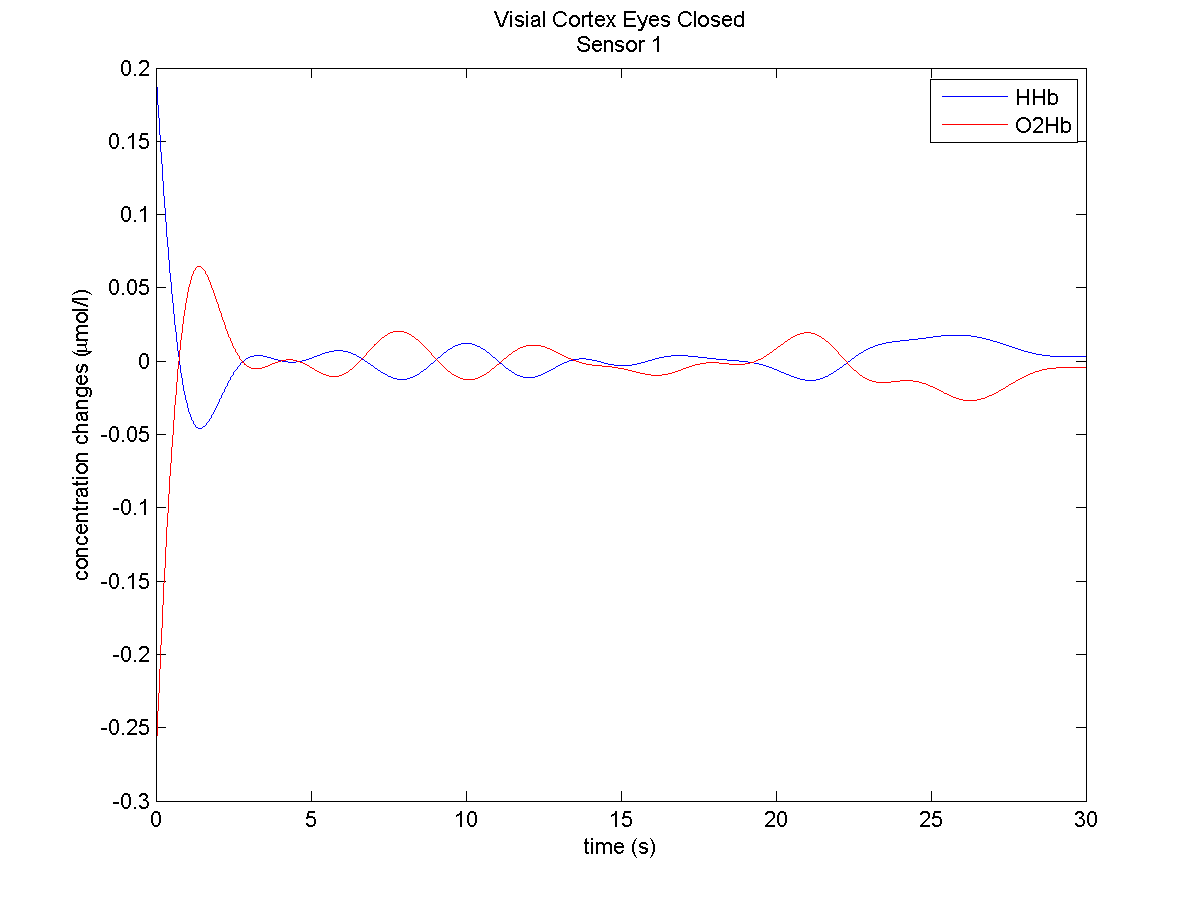
\includegraphics[width=4in]{VisialCortex-EyesClosed/sensor1.png}}
\subfigure[Sensor 2]{ 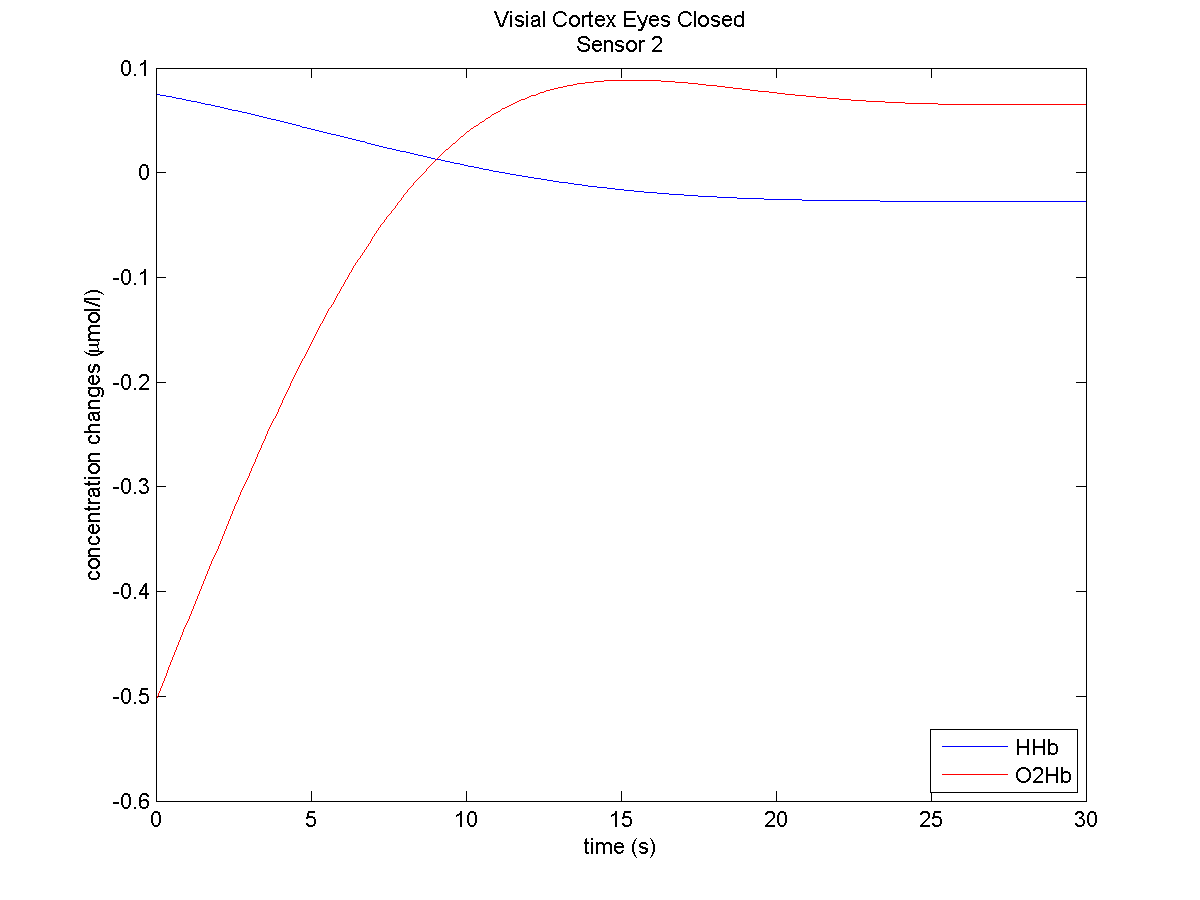
\includegraphics[width=4in]{VisialCortex-EyesClosed/sensor2.png}}
\caption[Frontal Lobe Measurements while Relaxed]{The result of having the subject close their eyes with the sensor placed over the visual cortex. The change in concentration of oxyhaemoglobin is marked in red and the change in concentration of deoxyhaemoglobin is marked in blue.}
\end{figure}

Interpreting these results is not quite clear. Even with the subject's eyes closed there seems to still be brain activity occurring in the visual cortex, though to a lesser degree than that when the subject's eyes were open. Perhaps there was movement of the sensor in the second measurements or possibly the subject was still moving their eyes with their eyes closed. 

Where the change in oxyhaemoglobin starts to increase and the change in deoxyhaemoglobin starts to increase in Figure 5.11 (with the subject's eyes open) is where the subject slowed down their eye movements and took longer to stare at each object. There is still brain activity occurring, but to a lesser degree than when the subject's eyes were moving fast, which is why there is a decrease in the change of oxygenation. This is a potential fatal flaw of this system. At this point it appears as if the subject closed their eyes or rather brain activity stopped occurring in this area. However, this was not the case, instead lower amount of oxygenation was required by the neuron. This is where a system that can exactly quantify the concentration would stand out from this system.

\section{Muscle Contractions}

As an addition to this project, the system was tested to see if it could measure muscle activity. Placing the sensor onto the test subject's bicep and having them continually flex and extend their bicep yields the result in Figure 5.13. Giving the subject a heavy weight and having them flex and extend their bicep again yields the result in Figure 5.14.

\begin{figure}[htp]
\centering
\subfigure[Sensor 1]{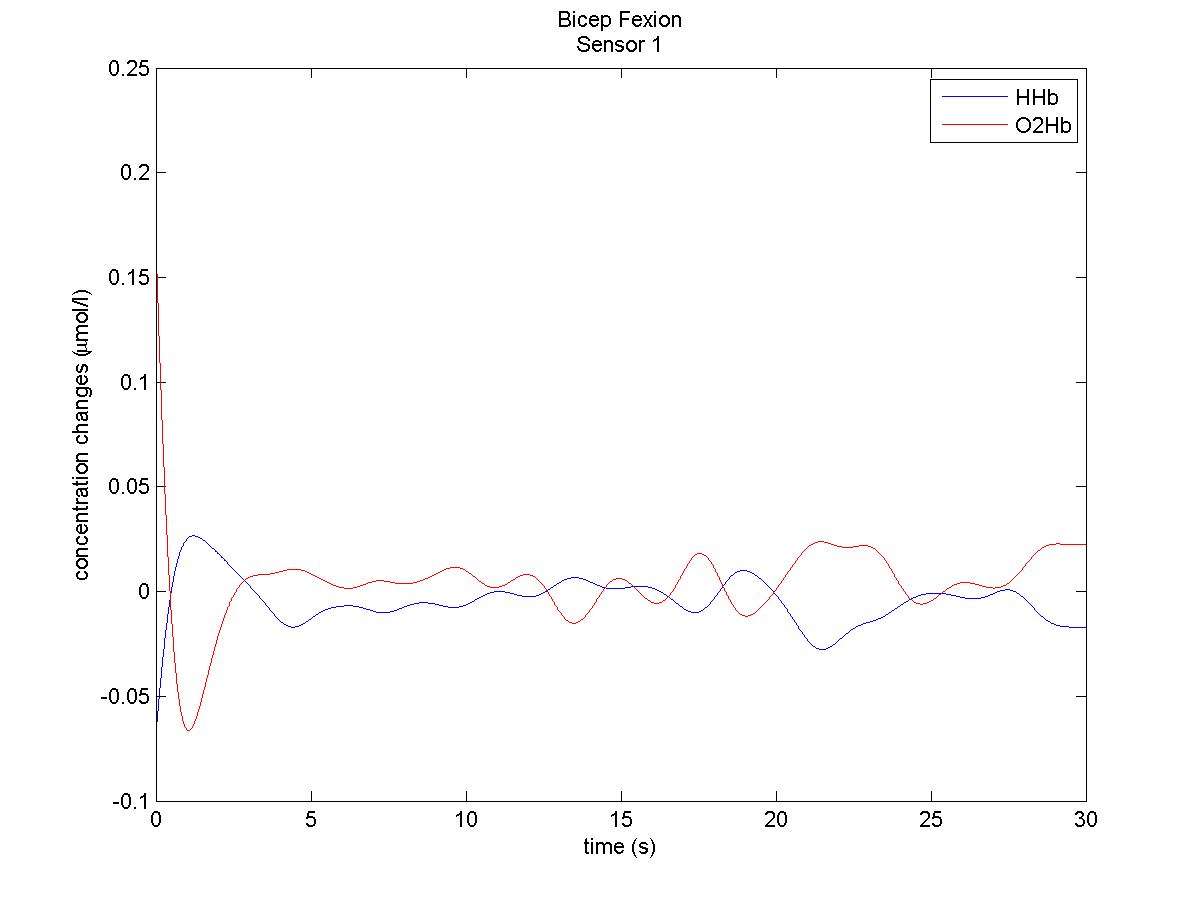
\includegraphics[width=4in]{BicepFexion/sensor1.png}}
\subfigure[Sensor 2]{ 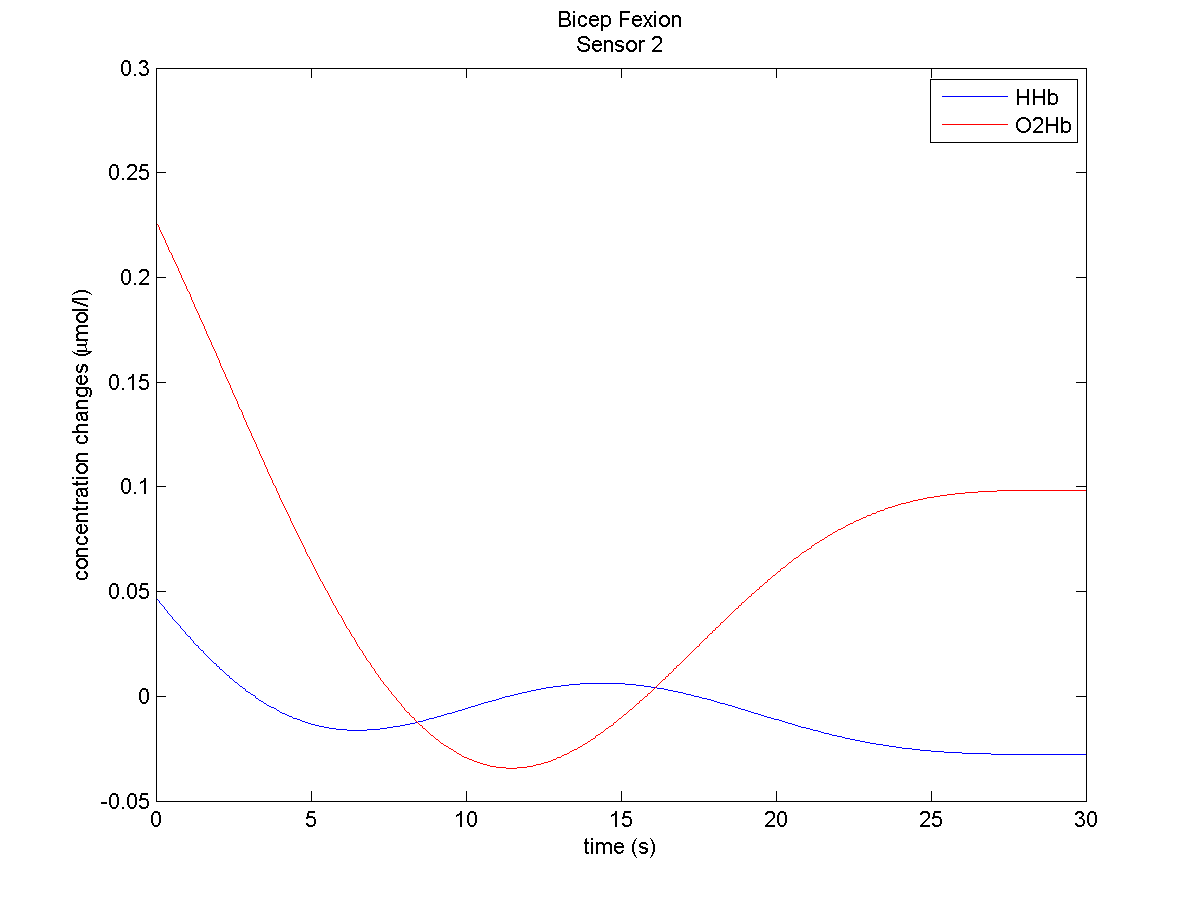
\includegraphics[width=4in]{BicepFexion/sensor2.png}}
\caption[Bicep Measurements with Continuous Flexion and Extension]{The result of having the subject continually flex and extend their bicep with the sensor placed over the bicep under activity. The change in concentration of oxyhaemoglobin is marked in red and the change in concentration of deoxyhaemoglobin is marked in blue. The subject stopped continuously flexing and extending their arm at around 8s, leaving it in the extended state until around 15s, where they began flexing and extending their bicep again}
\end{figure}


\begin{figure}[htp]
\centering
\subfigure[Sensor 1]{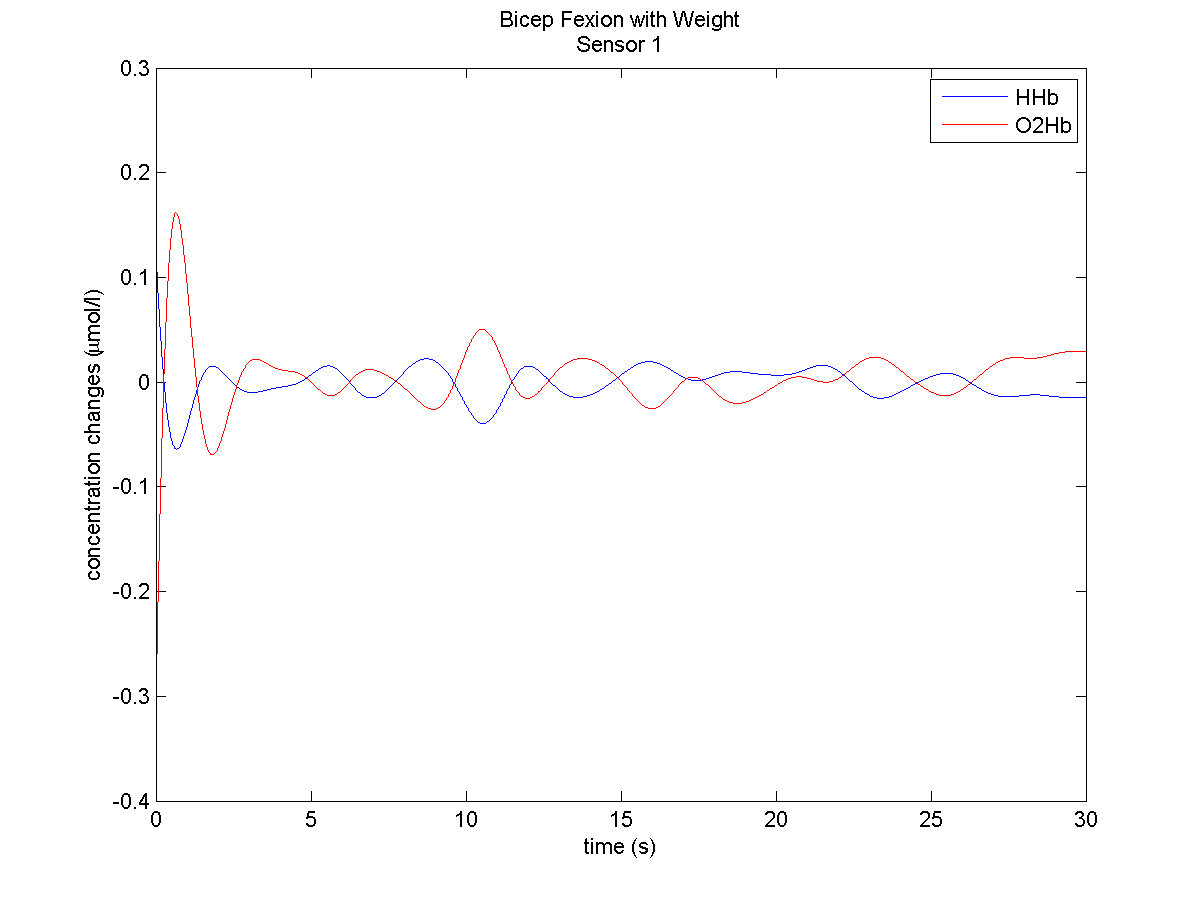
\includegraphics[width=4in]{BicepFexionWeight/sensor1.png}}
\subfigure[Sensor 2]{ 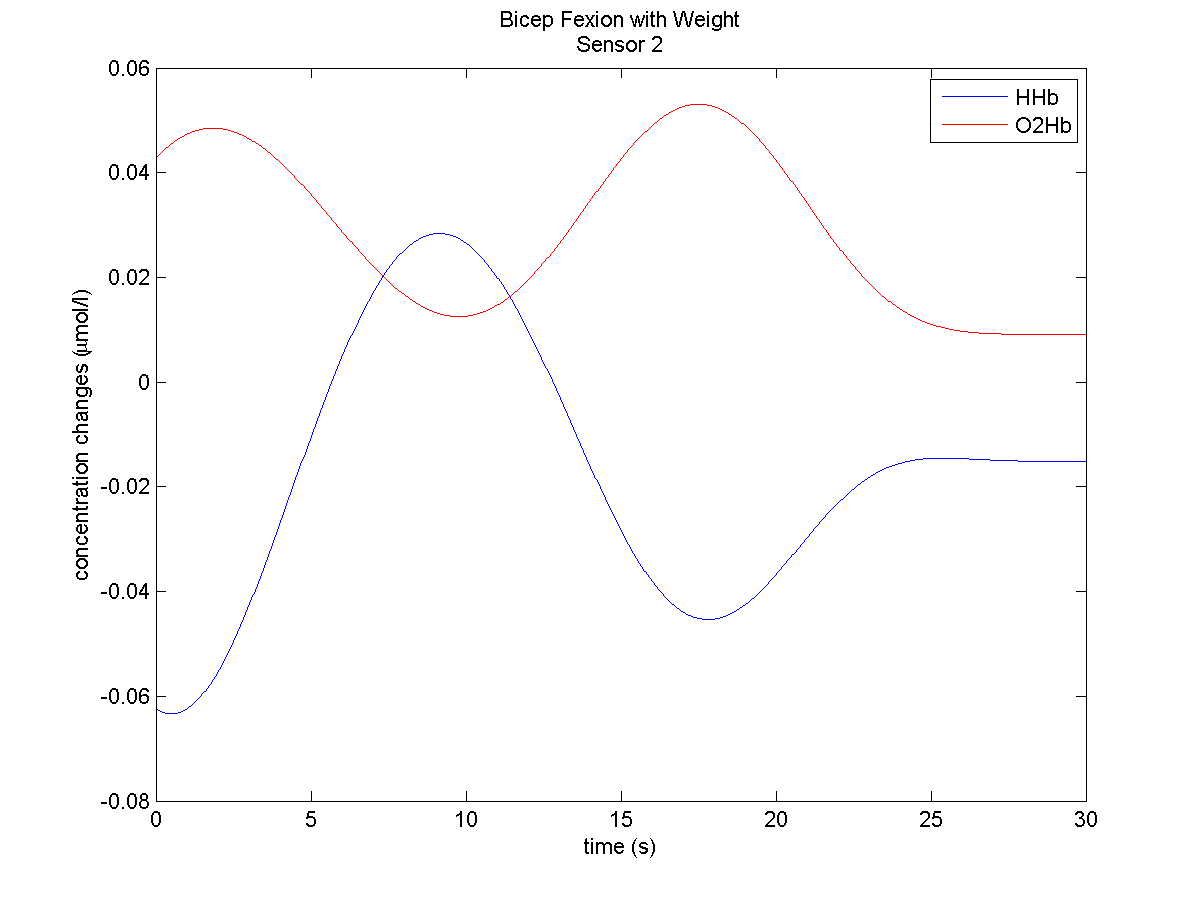
\includegraphics[width=4in]{BicepFexionWeight/sensor2.png}}
\caption[Bicep Measurements with Continuous Fexion and Extension with a Weight]{The result of having the subject continually flex and extend their bicep with a heavy weight in their hand with the sensor placed over the bicep under activity. The change in concentration of oxyhaemoglobin is marked in red and the change in concentration of deoxyhaemoglobin is marked in blue. The subject began lifting the weight at 0s, became fatigued at around 6s and was unable to lift the weight, began lifting the weight again at around 11s, finally becoming fatigued at around 23s. The subject still held the weight in their hand while fatigued, continually trying to lift it.}
\end{figure}

These results prove interesting, the system can indeed measure muscle activity. With the change in oxyhaemoglobin rates increasing during muscle activity and decreasing when not under activity, similar to brain activity. Interestingly, it can be seen that when trying to lift the wight the change in concentrations is higher than when not lifting any weight. This shows that when trying to lift more weight, the muscle has an increased need for oxygen. It can also be seen that when the muscle is fatigued, rather than having the change in oxyhaemoglobin decrease to below 0 and the change in deoxyhaemoglobin increase to above 0, the change in oxyhaemoglobin is constant and a positive value. Similarly, the change in deoxyhaemoglobin is constant and a negative value. This shows the muscle still requires oxygen and oxygenated blood is still coming in trying to restore the muscle to normal, while the muscle fibres are constantly consuming oxygen.

\section{Remarks}

This system is far from perfect. Every couple of measurements will result in one bad one that is either riddled with noise or does not make any sense. However, repeating the same measurement later on may yield positive results. It has not been determined what causes this. When the results are positive, they are repeatable, though.

The system has very good battery life. Granted it is powered by three AA batteries. Throughout the entire prototyping phase, the batteries were never needed to be changed. Previous systems have shown to have a battery life of just 3 hours \cite{rosen05}. The exact battery life of the system when constantly on is unknown, it should compete favourably with those previous systems though. The system has a ridiculously long standby time, having been in standby for at least 24hours. This is all due to the low power components in the system. 

While the prototype is not portable by all definitions of the word, it is battery powered and wireless and can be easy transported for use in the field. Due to the use of the breadboard the prototype is fairly large. However, should a PCB be made for the system, it could easily be made to be 6cm by 2cm, excluding the USB to UART module. At this size, the system wold definitely be portable by all definitions of the word. 
	\setcounter{figure}{0}
        \setcounter{equation}{0}
        \setcounter{table}{0}

  \chapter {Recommendations}

There are quite a few improvements that can be made to the system that were mainly not implemented due to time constraints and/or unexpected problems.

LED light and photodiode insulation is a topic that was not addressed in this system. To increase the SNR of the system it is advisable to block outside sources of light from interfering with the measurements or light sources. It is advisable to use some form of black insulation to absorb the outside light rather than reflect it to reduce scattering and increase SNR. 

One way of doing this is to apply black epoxy around the LEDs and photodiodes sufficiently to block light leakage and external light. However, sourcing medical grade black epoxy is not an easy task; it is hard enough finding normal black epoxy. It is possible to add a pigment to white epoxy, but this is no easy task either. An alternative is to use some kind of black foam or mesh.

The design of the sensor is not ideal. If it were to be revised a double-sided PCB would be used or the sensor would be made larger to reduce the number of jumper wires. This would help to make the sensor more robust and make building the sensor easier. Additionally the traces would be made larger to reduce the chance of breakage when flexed. 

The LEDs do not rest against the patient's skin when the sensor is placed against the patient. This reduced the SNR of the system by allowing light in from outside sources and decreases the light intensity before reaching the area of interest. This was the unattended side-affect of using SMD LEDs with the OPT101 monolithic photodiodes. Perhaps the use of standard SMD photodiodes or non-SMD LEDs would fix this. However, the use of standard SMD photodiodes would require the addition of a transimpedance amplifier. Finding non-SMD LEDs would be hard task, the SMD LEDs were selected in this project because that was all that could be acquired for a reasonable price. 

Attaching the sensors to the patients head was not addressed in this project. This is more or less a luxury. For the testing phase it is somewhat sufficient to hold the sensors to the head by hand. This will not be suitable for the final product though; any movement from the area of interest will add noise into the measurements. Thus, current ideas for achieving this would be using something like a headband or hairband to hold the sensor down; something that would provide enough pressure to ensure the sensor doesn't move while still allowing comfort for the patient.

Currently, this microcontroller uses BJTs to control the infrared LEDS. Should a second revision be done, an LED driver which controls the LEDs by PWM (pulse width modulation) would be used rather than simple BJTs. This will increase the efficiency of the system and allow greater control over the LEDs. This would allow for more localized measurements and power savings. Being able to control the brightness of the LEDs can be very advantageous for a versatile system. It does, however, come at the cost of complexity and thus time.

The overall system would greatly benefit if the system could display the data in real time. This is not very hard to do, just time consuming. Though having this would be of great benefit in a clinical environment where seeing the results the as fast possible may save life. 

Perhaps the greatest downfall of this project was trying to accomplish too much in a short period of time. The author took on the task of designing everything from scratch. This may have been detrimental to the overall result of the project. Rather than spending time on correctly displaying the results or ensuring the system work correctly all the time, time was spent make the microcontroller. It probably would have been beneficial to the project to have used an existing embedded system and focus more on the overall result. However, the knowledge gained has been invaluable to the author and the experience obtained designing the microcontroller will more likely be more beneficial to the author in the long run.

\chapter {Conclusion}

Despite these limitations, a fairly low-cost, wireless portable Near Infrared Spectrophotometry system was successfully built that is able to measure haemodynamic signals. The results shown by the NIRS device created in this project are promising. It was able to measure brain activity in the brain not only during motor activity, but during intense thinking and visual stimulation. The results are fairly promising as well, there is a strong correlation between brain activity and the measurements taken. In addition, it is also able to directly measure muscle activity, which was an unexpected bonus. 

While NIRS devices are currently still in the research phase with very few commercial systems, it is hard to see it ever successfully replacing EEG or fMRI measurements. EEG systems have a very large marketshare with commercially available system everywhere for very cheap and have a slightly higher temporal resolution than NIRS. fMRI has a much higher spatial resolution than NIRS, at the cost of temporal resolution, but there are many times researchers or doctors need to see brain activity deep into the brain. Laser NIRS systems can penetrate deeper than LED based ones, but at an increased cost, complexity, and loss of portability. However, there is that niche market where EEG does not cut it due to electromagnetic interference or a device with spatial resolution is required but fMRI is deemed to costly, is unable to be used due to long waiting lists, or in the case the patient cannot be transferred to the MRI machine. For this niche market, NIRS is their saviour.                   % the first chapter
        \setcounter{figure}{0}
        \setcounter{equation}{0}
        \setcounter{table}{0}

 \appendix

\chapter {Calculations}

\section {Minimum UART speed calculation}

Given 2 sensors and a time resolution of 10ms (refer to Figure 4.9),

\begin{equation}
\frac{10\ ms}{12\ parts} \div 4\ parts = 4800\ Hz
\end{equation}
\begin{equation}
\frac {4800} {s} \times 16\ bits = 76\ 800\ bit/s
\end{equation}

\section {DPF calculation}

The differential path length factor (DPF) can be calculated from the following equation \cite{rosen05}

\begin{equation}
DPF^\lambda = \frac{1}{2}\left(\frac{3\mu_{s}^\lambda}{\mu_{a}^\lambda}\right)^{1/2} \left(1-\frac{1}{1+d(3\mu_{s}^\lambda\mu_{a}^\lambda)^{1/2}}\right)
\end{equation}

The absorption ($\mu_{a}^\lambda$) and reduced scattering ($\mu_{s}^\lambda$) coefficients cannot be directly measured by near infrared light, so the values given in past studies will be used. Specifically, $\mu_{a}^{730nm}$=0.015 mm$^{-1}$, $\mu_{a}^{850nm}$ = 0.023 mm$^{-1}$, $\mu_{s}^{730nm}$= 0.80 mm$^{-1}$, and $\mu_{s}^{850nm}$=0.95 mm$^{-1}$. The values at 750nm could not be found, so the values at 730nm will be used. Plugging these values into the equation above gives, $DPF^{730nm}$=5.0055 and $DPF^{850nm}$=4.6564.

\chapter{Flow Charts}
\section {Microcontroller code flow chart}

\headsep = 5pt
\begin{figure}[htp]
\centering
\caption{Microcontroller code flow chart}
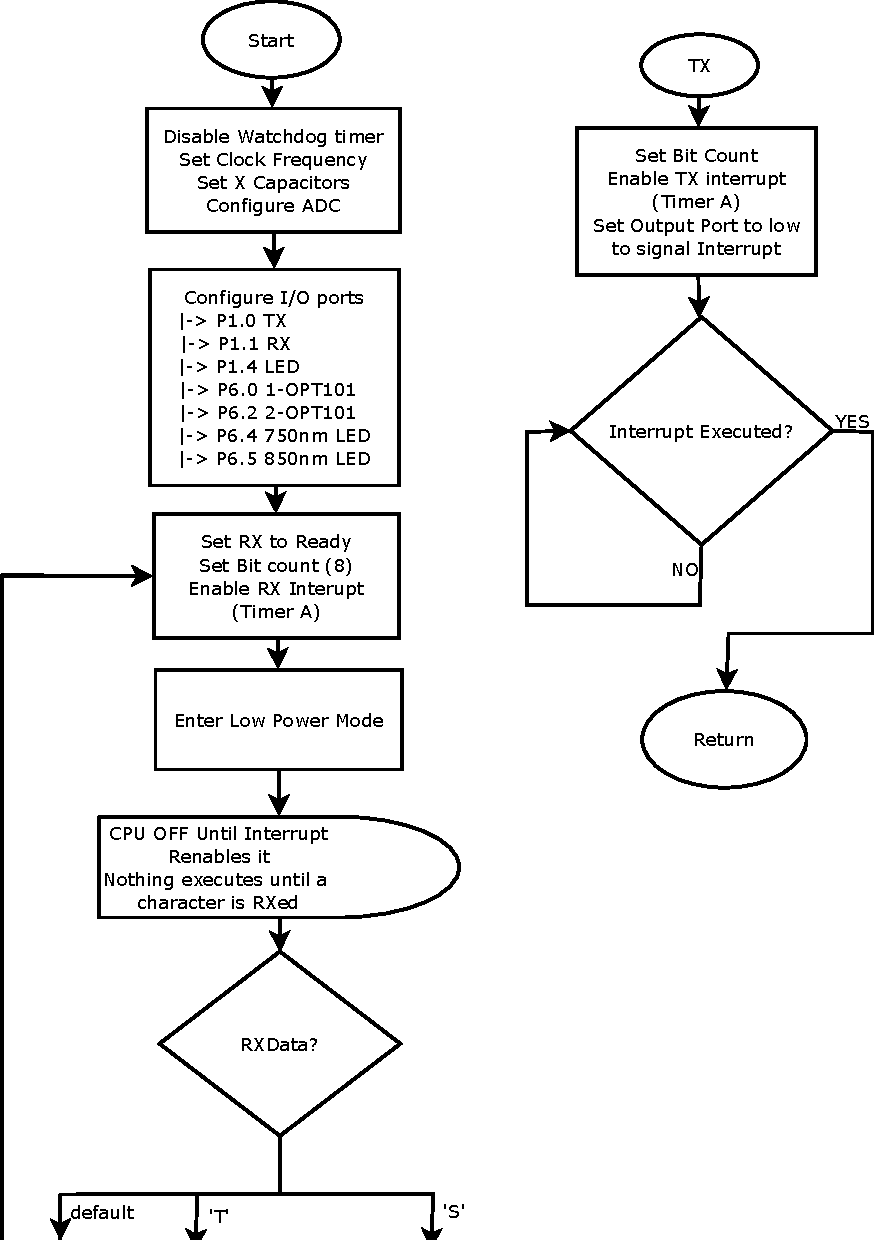
\includegraphics[height=8.05in]{cdia-1.pdf}
\end{figure}

\begin{figure}[htp]
\centering
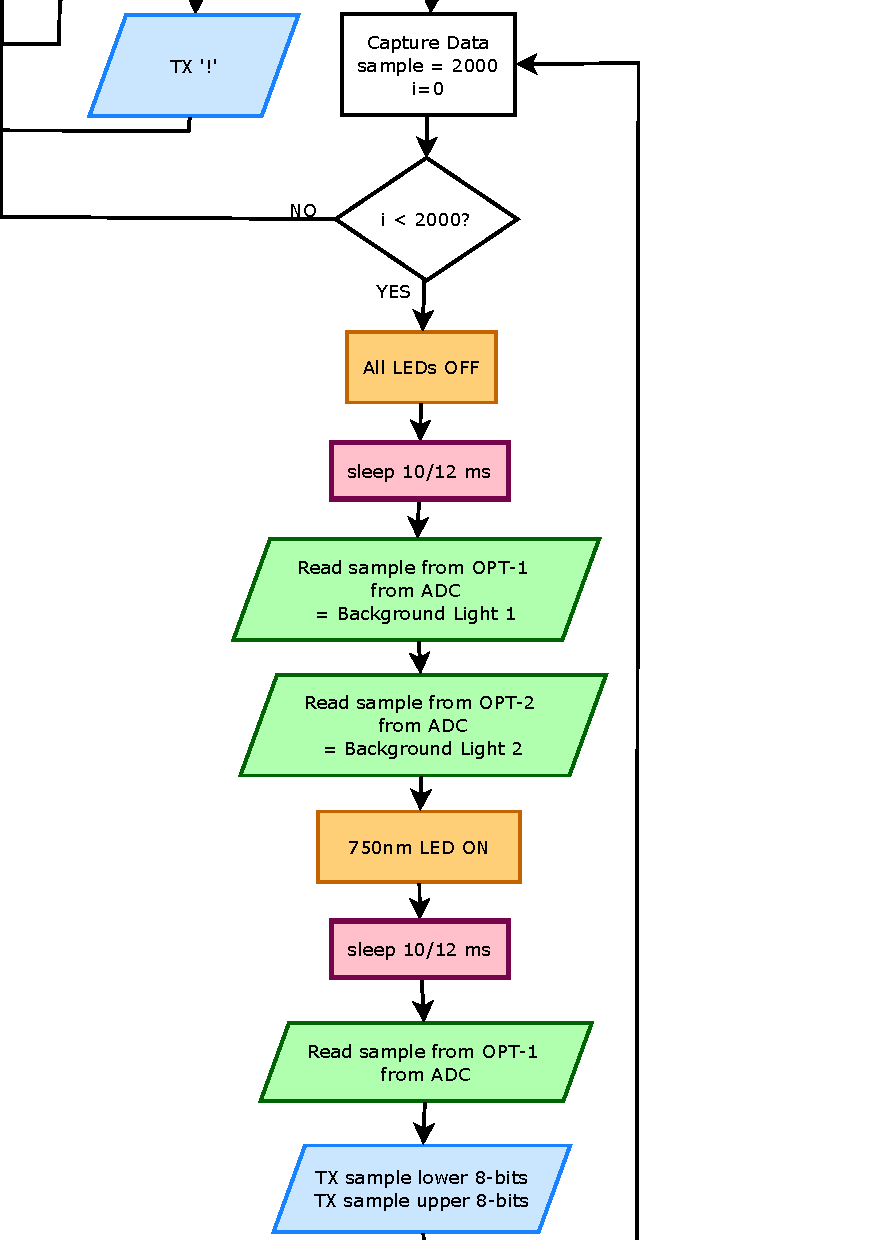
\includegraphics{cdia-2.pdf}
\end{figure}

\begin{figure}[htp]
\centering
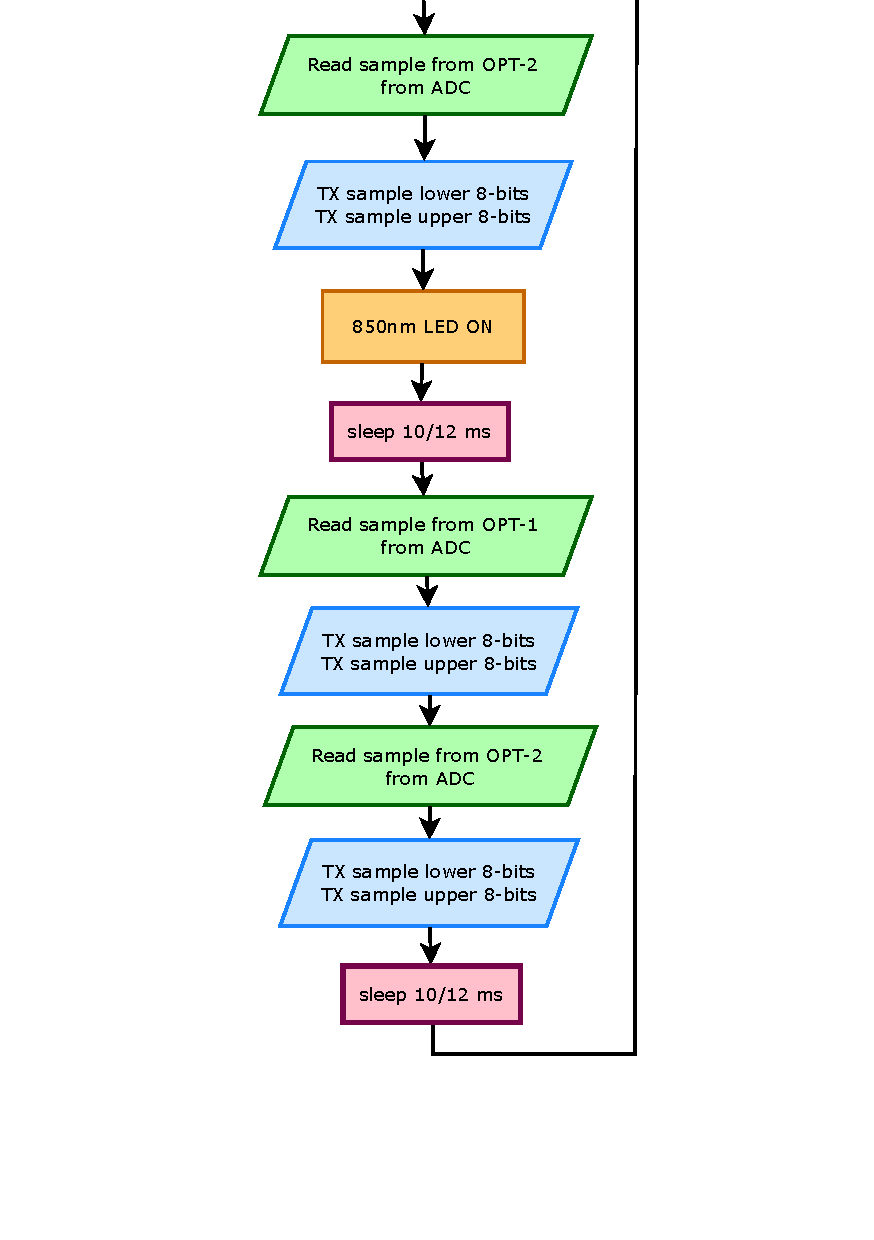
\includegraphics{cdia-3.pdf}
\end{figure}

\begin{figure}[htp]
\centering
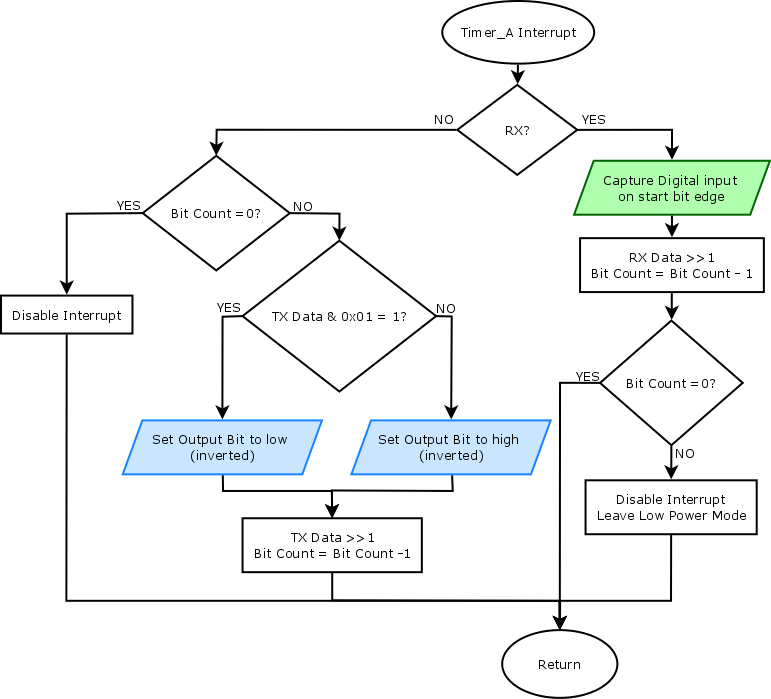
\includegraphics[width=6in]{cdiatimer.png}
\caption{Timer\_A interrupt flow chart}
\end{figure}

\headsep = 0.5in

\chapter {Matlab Source Code}
\lstinputlisting[language=Matlab,breaklines=true]{filter.m}               % you can include your appendix if you have any!\

%\bibliographystyle{ieeetr}
\bibliography{references}        % your list of references

\chapter*{Vita}

\begin{center}
\begin{tabular}{rl}
  \sc Name: &Sukneet Basuta, formally Sukneet Saini \\
  \sc Place of Birth:&Ottawa, Canada\\
  \sc Secondary Education:&John Mccrae Secondary School (2005)\\
  \sc Honours and Awards:&McMaster Entrance Scholarship 2005
\end{tabular}
\end{center}

\label{NumDocumentPages}

\end{document}
% ********************************
